\documentclass[c]{beamer}
%\documentclass[c,aspectratio=1610]{beamer}
\mode<presentation>
{
  \usetheme[progressbar=frametitle]{metropolis}       % or try default, Darmstadt, Warsaw, Darmstadt ,Berkeley,...
  \usecolortheme{default} % or try albatross, beaver, crane,whale,orchid,spruce,...
  \usefonttheme{serif}    % or try default, structurebold,serif ...
  \setbeamertemplate{navigation symbols}{}
  \setbeamertemplate{caption}[numbered]
  \setbeamercovered{transparent}
} 
\addtobeamertemplate{block begin}{\pgfsetfillopacity{0.8}}{\pgfsetfillopacity{1}}
\addtobeamertemplate{block alerted begin}{\pgfsetfillopacity{0.8}}{\pgfsetfillopacity{1}}
\addtobeamertemplate{block example begin}{\pgfsetfillopacity{0.8}}{\pgfsetfillopacity{1}}

%\usepackage{beamerthemesplit}
%\usepackage[orientation=landscape,size=custom,width=14.5,height=8,scale=0.30,debug]{beamerposter}
%\usepackage[orientation=landscape,size=custom,width=18.0,height=10.0,scale=0.40,debug]{beamerposter} 


\usepackage[T1]{fontenc}
\usepackage[utf8]{inputenc}
\usepackage[brazil]{babel}
\usepackage[brazilian,hyperpageref]{backref}
\usepackage[scale=2]{ccicons}
\usepackage{pgfplots}
\usepackage{braket}
\usepackage{cancel}
\usepgfplotslibrary{dateplot}
\usefonttheme{serif}
% \usepackage{ebgaramond}
%\usepackage{palatino}
%\usepackage{kpfonts}
%\usepackage{times}
%\usepackage{xspace}
% \usepackage{natbib}
% \usepackage{cite}
\usepackage{mathtext}
\usepackage{amsfonts,amssymb}
\usepackage{amsmath,amsthm}
\usepackage{epsfig,epstopdf,url,array,latexsym}
\usepackage{graphicx}
\usepackage{mathrsfs}
\usepackage{natbib}
\usepackage{float}
\usepackage{caption}
\usepackage{subcaption}
\usepackage[mathcal]{euscript}
\usepackage{esvect}
\captionsetup[figure]{labelfont=sc}
 \usepackage{microtype} 
 \usepackage{multicol}
 \usepackage{multirow}
\usepackage{longtable}
\usepackage{lscape}
\usepackage{booktabs}
\usepackage{verbatim}
\usepackage{cprotect}
\usepackage[subnum]{cases}
\usepackage{physics}
\newcommand{\themename}{\textbf{\textsc{metropolis}}\xspace}
\title{{\sc Introdução ao \LaTeX}}
%\subtitle{X Semana Acadêmica da Física\\
%	Diretório Acadêmico César Lattes}
\subtitle{Módulo 2: Ambientes em geral, figuras e tabelas.}
\date{\today}
\author{	{\large XI Semana Acadêmica da Física}\\
	Fernanda Vanucci {\sc Sica}\inst{1}\footnote{\texttt{fervanucci@gmail.com}},
	Geferson {\sc Lucatelli}\inst{1}\footnote{\texttt{gefersonlucatelli@gmail.com\\[0.5cm]}}}
\institute{{\Large Universidade Federal do Rio Grande} \\[0.3cm]
	{\inst{1}\large Instituto de Matemática, Estatística e Física
	}}
\titlegraphic{\hfill
	
\includegraphics[height=1.5cm]{images/furg.png}\\[2.5cm]{
\hspace*{8cm}
\includegraphics[height=1.5cm]{images/imef2.png}}
\hspace*{8.5cm}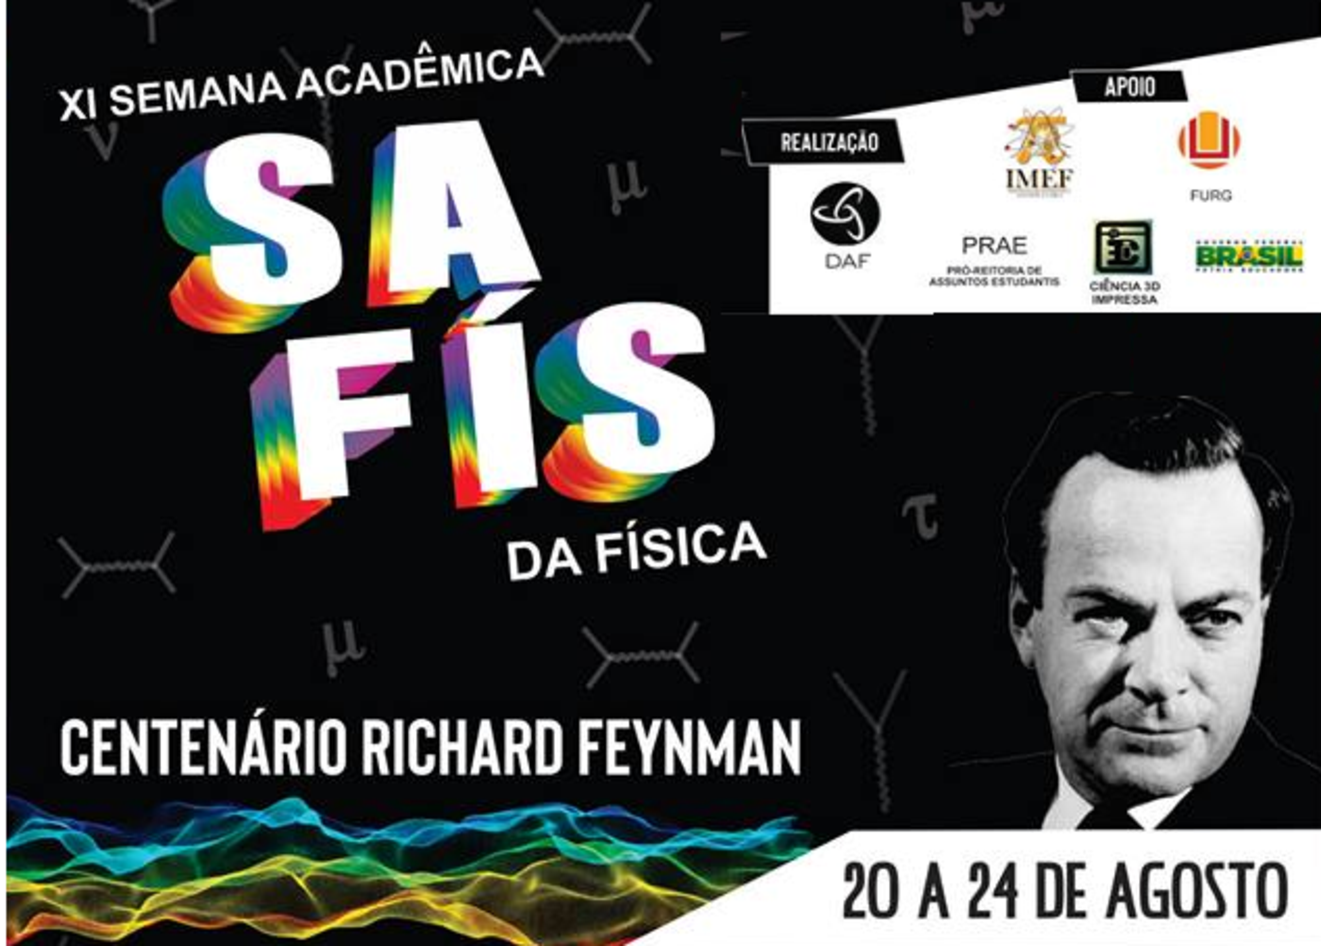
\includegraphics[height=2.0cm]{images/safis2018.pdf}
}
% \logo{
\includegraphics[scale=.04]{images/furg.png} / 
% 	
\includegraphics[scale=.03]{images/imef2.png}}
\newcommand{\qv}[1]{\widetilde{ #1 }}
\renewcommand{\r}{\right}
\renewcommand{\l}{\left}
\newcommand*{\EE}{\mathscr{E}}
\newcommand*{\BB}{\mathscr{B}}
\newcommand*{\Hh}{\mathscr{H}}
\newcommand*{\D}{{\rm d}}
\newcommand*{\PP}{\mathscr{P}}
\newcommand*{\WW}{\mathcal{W}}
\newcommand*{\A}{\mathscr{A}}
%\renewcommand*{\partial}{
\includegraphics[scale=0.08]{partial_symb.pdf}}%
\renewcommand*{\vec}{\vv}%
% \renewcommand{\vec}[1]{\vv{ #1 }}

\newcommand*{\ii}{\mathfrak{i}}
% \newcommand*{\prt}{\includegraphics[scale=0.40]{partial_symbol.pdf}}%
\newcommand{\source}[1]{
% \begin{flushleft}
\caption*{Fonte: {#1}} 
% \end{flushleft}
}
% \bibliographystyle{apasoft}
\bibliographystyle{apalike}
\setbeamertemplate{section in toc}{\hspace*{1em}\inserttocsectionnumber.~\inserttocsection\par}
\setbeamertemplate{subsection in toc}{\hspace*{2em}\inserttocsectionnumber.\inserttocsubsectionnumber.~\inserttocsubsection\par}
\setbeamercovered{invisible}
\usepackage{xpatch}

\usepackage{ragged2e}
\usepackage{etoolbox}
\apptocmd{\frame}{}{\justifying}{}
%\xpatchcmd{\itemize}
%{\def\makelabel}
%{\setlength{\itemsep}{5ex}\def\makelabel}
%{}
%{}
\usepackage{cleveref}
\usepackage{adjustbox}
\begin{document}
\maketitle


{\fontsize{9pt}{10.0}\selectfont

\begin{frame}{\sc Sumário}
	\begin{multicols}{2}
			\tableofcontents
	\end{multicols}
%  \setbeamertemplate{section in toc}[sections numbered]
%  \tableofcontents[section,subsection]
% \tableofcontents[hideallsubsubsections]
%   \tableofcontents[hideallsubsubsections]
\end{frame}
}
%%%%%%%%%%%%%%%%%%%%%%%%%%%%
%
%\begin{frame}
%	\begin{center}
%		{\Huge Parte 2}
%	\end{center}
%\end{frame}

{\fontsize{10pt}{10.0}\selectfont
%\section{Introdução as nebulosas gasosas}


\section{Ambientes}
\plain{Para que servem os ambientes?}


%\begin{frame}[fragile]{\sc Ambientes: \texttt{document}}
%	\begin{itemize}
%		\setlength\itemsep{0.3cm}
%		\item ambientes $:\to$ \verb|environment| são utilizados 
%		para inúmeras funções;
%		\item para iniciar e fechar um ambiente, se utiliza 
%		\begin{verbatim}
%		\begin{environment}
%		...
%		\end{environment}		
%		\end{verbatim}
%		\item o ambiente raiz de todo o texto é o \verb|document|. 
%		Tudo o que estiver entre
%		\begin{verbatim}
%		\begin{document}
%		...
%		\end{document}
%		\end{verbatim}
%		será o texto a ser produzido;
%		\item demais ambiantes serão vistos ao longo do curso;
%	\end{itemize}
%\end{frame}

\begin{frame}[fragile]{\sc Ambientes}
Um {\color{blue} ambiente} é uma região do texto que tem um tratamento especial.  
Um ambiente é {\color{blue} iniciado} com \verb|\begin{}| e {\color{blue} terminado} com 
\verb|\end{}|, onde o nome do ambiente está entre as chaves. {\color{blue} Exemplos} de ambientes são:
\begin{itemize}
	\setlength\itemsep{0.1cm}
	\item Listas
	\begin{itemize}
		\item \verb|itemize|
		\item \verb|enumerate|
	\end{itemize}
	\item Alinhamento
	\begin{itemize}
		\item \verb|\flushleft|
		\item \verb|\flushright|
		\item \verb|\center|
	\end{itemize}
	\item Matemático
	\begin{itemize}
		\item \verb|equation|
		\item \verb|eqnarray|
		\item \verb|align|
	\end{itemize}
	\item Tabelas
	\item Figuras
\end{itemize}
\end{frame}

\subsection{Listas}
\subsubsection{Listas por itens}
\plain{Ambientes de listas por itens.}

\begin{frame}[fragile]{\sc Listas por itens - \texttt{itemize}}
Os ambientes de {\color{blue} listas} possuem o mesmo modelo de código.
\begin{verbatim}
\begin{ambiente_de_lista}
\item texto
\item texto
\end{ambiente_de_lista}
\end{verbatim}
\end{frame}




\begin{frame}[fragile]{\sc Listas por itens - \texttt{itemize}}
	\center{{\color{blue} Exemplo de lista} utilizando o ambiente \verb|itemize|:}
	\begin{columns}
		\begin{column}[t]{0.5\textwidth}
			\begin{itemize}
				\setlength\itemsep{0.3cm}
				\item Primeiro item
				\item Segundo item
				\item Terceiro item
			\end{itemize}
		\end{column}
		
		\begin{column}[t]{0.5\textwidth}
		\begin{verbatim}
			\begin{itemize}
			\item Primeiro item 
			\item Segundo item 
			\item Terceiro item
			\end{itemize}
		\end{verbatim}
		\end{column}
		
	\end{columns}
	
\end{frame}

\begin{frame}[fragile]{\sc Sublistas - \texttt{itemize}}
	\center{Exemplo de {\color{blue} sublista}:}
	\vspace{0.2cm}
	\begin{columns}
		\begin{column}[t]{0.5\textwidth}
			\begin{itemize}
				\item Primeiro item
				\begin{itemize}
					\setlength\itemsep{0.3cm}
					\item Primeiro subitem
					\item Segundo subitem
				\end{itemize}
				\item Segundo item
			\end{itemize}
		\end{column}
		
		\begin{column}[t]{0.5\textwidth}
			\begin{verbatim}
			\begin{itemize}
			\item Primeiro item
				\begin{itemize}
				\item Primeiro subitem
				\item Segundo subitem
				\end{itemize}
			\item Segundo item
			\end{itemize}
			\end{verbatim}
		\end{column}
		
	\end{columns}
	
\end{frame}

\subsubsection{Lista ordenadas}
\plain{Ambientes de listas ordenadas}

\begin{frame}[fragile]{\sc Listas ordenadas - \texttt{enumerate}}
	O ambiente \texttt{enumerate} gera {\color{blue} listas numeradas}.	
	\begin{columns}
		\begin{column}[t]{0.5\textwidth}
			\begin{enumerate}
				\item Primeiro item
				\item Segundo item
				\item Terceiro item
			\end{enumerate}
		\end{column}
		%
		\begin{column}[t]{0.5\textwidth}
			\begin{verbatim}
			\begin{enumerate}
			\item Primeiro item
			\item Segundo item
			\item Terceiro item
			\end{enumerate}
			\end{verbatim}
		\end{column}
		
	\end{columns}
	
\end{frame}

\begin{frame}[fragile]{\sc Sublistas ordenadas}
	Também é possível gerar {\color{blue} sublistas ordenadas}.
	
	\begin{columns}
		\begin{column}[t]{0.5\textwidth}
			\begin{enumerate}
				\item Primeiro item
				\begin{enumerate}
					\item Primeiro subitem
					\item Segundo subitem
				\end{enumerate}
				\item Segundo item
			\end{enumerate}
		\end{column}
		
		\begin{column}[t]{0.5\textwidth}			
			\begin{verbatim}
			\begin{enumerate}
			\item Primeiro item
				\begin{enumerate}
				\item Primeiro subitem
				\item Segundo subitem
				\end{enumerate}
			\item Segundo item
			\end{enumerate}
			\end{verbatim}
		\end{column}
	\end{columns}
	
\end{frame}

\begin{frame}[fragile]{\sc Mais sobre o \texttt{enumerate}}
	O ambiente \texttt{enumerate} nos permite controlar o 
	{\color{blue} formato da lista}. 
	Para isto, precisamos adicionar no preambulo o pacote,
\begin{verbatim}
\usepackage{enumerate}
\end{verbatim}	
	a modificação é feita ao iniciar o ambiente, da seguinte forma,
\begin{verbatim}
\begin{enumerate}[opção]
\end{verbatim}	
onde as opções podem ser:
	\begin{enumerate}[i)]
		\item \verb|i)|
	\end{enumerate}
	\begin{enumerate}[(i)]
		\item \verb|(i)|
	\end{enumerate}
	\begin{enumerate}[I)]
		\item \verb|I)|
	\end{enumerate}
	\begin{enumerate}[(a)]
		\item \verb|(a)|
	\end{enumerate}
\end{frame}

\begin{frame}[fragile]{\sc Listas - Exercício}
	\underline{Reproduzir a lista abaixo!}
	    \begin{enumerate}[1)]
	    	\item Primeiro item
	    	\begin{enumerate}[i)]
	    		\item Primeiro subitem
	    		\begin{itemize}
	    			\item primeiro subsubitem
	    		\end{itemize}
	    		\item Segundo subitem
	    		\begin{itemize}
	    			\item segundo subsubitem
	    		\end{itemize}
	    	\end{enumerate}
	    	\item Segundo item
	    \end{enumerate}
\end{frame}

\begin{frame}[fragile]{\sc Listas - Exercícios (solução)}
\begin{verbatim}
	    \begin{enumerate}[1)]
	    \item Primeiro item
		        \begin{enumerate}[i)]
		        \item Primeiro subitem
			            \begin{itemize}
			            \item primeiro subsubitem
			            \end{itemize}
		        \item Segundo subitem
			            \begin{itemize}
			            \item segundo subsubitem
			            \end{itemize}
		        \end{enumerate}
		    \item Segundo item
		    \end{enumerate}
\end{verbatim}
\end{frame}


\subsection{Alinhamento}
\plain{Ambientes de alinhamento}

\begin{frame}[fragile]{\sc Alinhamento}
	Normalmente o \LaTeX \ mantêm os textos com o alinhamento ``justificado''. 
	Para {\color{blue} modificar o alinhamento}, podemos utilizar 3 opções:
	\begin{itemize}
		\setlength\itemsep{0.3cm}
		\item \verb|flushleft|, alinhado à esquerda;
		\item \verb|flushright|, alinhado à direita;
		\item \verb|center|, centralizado.
	\end{itemize}
	O {\color{blue} código} para utilizar estes alinhamento é o seguinte,
	
	\begin{verbatim}
	\begin{alinhamento}
	texto, frase ou parágrafo
	\end{alinhamento}
	\end{verbatim}
\end{frame}

\subsection{Expressões Matemáticas}
\plain{Uma das principais utilidades do \LaTeX\ vem agora.\\
	Expressões matemáticas!}


\begin{frame}[fragile]{\sc Expressões Matemáticas}
	Como escrever uma expressão matemática como abaixo? 
	\begin{align}
	x_H(t)=x_H(0)\cos\l(\omega t\r)+\frac{1}{m\omega}\underbrace{\l[
		\frac{\ii e^{-\ii\omega t}}{2}-\frac{\ii e^{\ii\omega t}}{2}
		\r]}_{\sin\l(\omega t\r)}
	p_H(0)
	+\frac{q\mathcal{E}}{2m\omega^2}\l(1-e^{-\ii\omega t}\r)
	\nonumber
	\end{align}
	\begin{itemize}
		\setlength\itemsep{0.3cm}
		\item lembando que para usar {\color{blue} ambientes matemáticos}, é preciso {\color{blue} adicionar} os 
		{\color{blue} pacotes} \verb|amsmath| e \verb|amssymb| ao preâmbulo;
	   \item {\color{blue} chaves} são interpretadas como {\color{blue} delimitadores de grupo}
	    e para serem impressas devem estar acompanhadas com \verb|\|,
	   ou seja, escrevemos \verb|\{ \}| ;  
	   \item espaços em branco são ignorados pelo compilador;
	   \item como padrão, todas as letras são escritas em itálico.
	\end{itemize}
\end{frame}

\begin{frame}[fragile]{\sc Expressões Matemáticas}
O {\color{blue} alfabeto grego} é largamente utilizado para {\color{blue} escrever equações}.
A seguir, apresentamos uma lista de caracteres do alfabeto e o respectivo comando:
\begin{figure}[h]
	\centering
	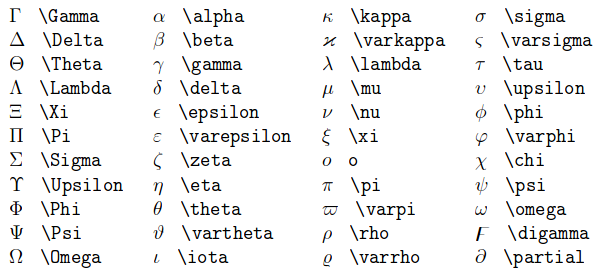
\includegraphics[scale=0.46]{images/letras_gregas.png}
\end{figure}
\end{frame}



\begin{frame}[fragile]{\sc Expressões Matemáticas: ambientes ``\texttt{\$\$ \$\$}'' e \texttt{equation}}
	\begin{itemize}
		\setlength\itemsep{0.3cm}
	   \item As equações matemáticas podem ser escritas de maneiras diferentes:
	   \begin{itemize}
	   	\item O comando \verb|$x+1=1$| produz $x+1=1$ (insere no texto);
	   	\item O comando \verb|$$x+1=1$$| produz (insere em uma linha separada) $$x+1=1;$$
	   	\item O comando \\
	   	\verb|\begin{equation}|\\
	   	\verb|x+1=1|\\
	   	\verb|\end{equation}|\\  
	   	produz 
	   	\begin{equation}
	   	x+1=1;
	   	\end{equation}
	   	\item o comando {\color{blue} ``\verb|$$ $$|''} insere equações rápidas {\color{blue} sem enumerá-las}, 
	   	já com o ambiente {\color{blue} \verb|equation|}, elas são {\color{blue} enumeradas};
	   \end{itemize}
	\end{itemize}
\end{frame}



\begin{frame}[fragile]{\sc Expressões Matemáticas: ambiente \texttt{align}}
	\begin{itemize}
		\setlength\itemsep{0.3cm}
		\item o ambiente \verb|align| permite escrever {\color{blue} múltiplas} linhas de {\color{blue} quações}; 
		\item é muito útil quando se quer resolver passo a passo uma equação!;
		\item por exemplo,
		     \begin{align}
		     f(x) & = 2x^{5} + 3x^{4} + x^{3}\nonumber\\
		     & \qquad + 2x^{2} + 5x + 8 \\
		     & = g(x) - h(x)
		     \end{align} 
		produz 
		\begin{verbatim}
		     \begin{align}
		     f(x) & = 2x^{5} + 3x^{4} + x^{3}\nonumber\\
		     & \qquad + 2x^{2} + 5x + 8 \\
		     & = g(x) - h(x)
		     \end{align} 
		\end{verbatim}
		\item toda a equação se {\color{blue} alinha verticalmente} com base no carácter\\
	 que acompanha o {\color{blue} símbolo \verb|&|}.
	\end{itemize}
\end{frame}


\plain{Como construir as equações?}

\begin{frame}[fragile]{\sc Índices e expoentes}
	\begin{itemize}
		\setlength\itemsep{0.2cm}
   \item Para criar {\color{blue} expoentes} e {\color{blue} sub-índices}, 
   utilizamos os comandos \verb|^| e \verb|_|, respectivamente;
   \item Exemplo: Escrevendo \\
   \begin{verbatim}
   \begin{equation*}
   \sum_{i = 1}^{n},\quad \prod_{i = 1}^{n}
   \end{equation*}
   \end{verbatim}
   obtemos
   \begin{equation*}
   \sum_{i = 1}^{n}, \quad  \prod_{i = 1}^{n}
   \end{equation*}
   \item o uso de ``\verb|*|'' após \verb|equation| {\color{blue} revome a enumeração} da equação;
   \item o mesmo se aplica para o ambiente \verb|align|;
   \item para inserir somatórias com múltiplos índices, use 
   \begin{align}
   \sum_{\substack{ i\neq j\\ j=1}}
   \end{align}
	\end{itemize}
\end{frame}



\begin{frame}[fragile]{\sc Índices e expoentes}
	\begin{itemize}
		\setlength\itemsep{0.2cm}
    \item Para inserir somatórias com múltiplos índices,
   \begin{align}
   \sum_{\substack{ i\neq j\\ j=1}}
   \end{align}
   use 
   \begin{verbatim}
   \begin{align}
   \sum_{\substack{ i\neq j\\ j=1}}
   \end{align}   
   \end{verbatim}
   \item índices ou expoentes compostos devem ser inseridos dentro do 
   delimitador \verb|{}|. Por exemplo, 
   \begin{verbatim}
   \begin{align*}
   e^{-x^2 -y^2}, \quad T_{x,y}
   \end{align*}
   \end{verbatim}
   produz 
   \begin{align*}
   e^{-x^2 -y^2}, \quad T_{x,y}
   \end{align*}
	\end{itemize}
\end{frame}

\begin{frame}[fragile]{\sc Frações}
	\begin{itemize}
		\setlength\itemsep{0.3cm}
   \item {\color{blue} Frações} são criadas utilizando os comandos \verb|\frac{numerador}{denominador}| 
   e raízes com \verb|\sqrt[n]{radicando}|;
   \item Exemplo: Escrevendo
   \begin{verbatim}
   \begin{align*}
   \frac{\sqrt[3]{xy}}{2}, \qquad\frac{\sqrt{xy}}{2}
   \end{align*}
   \end{verbatim}
   obtemos 
   \begin{align*}
   \frac{\sqrt[3]{xy}}{2}, \qquad \frac{\sqrt{xy}}{2}
   \end{align*}
   \item {\color{blue} frações} inseridas ao longo do {\color{blue} texto} ou dentro de um numerador/denominador 
   são reduzidas em tamanho, como por exemplo $\frac{x}{y}$, mas podem ser ajustadas usando o comando \verb|\cfrac{num}{den}|, 
   assim fica $\cfrac{x}{y}$;
	\end{itemize}
\end{frame}
	


\begin{frame}[fragile]{\sc Limites}
	\begin{itemize}
		\setlength\itemsep{0.3cm}
	   \item Para escrever {\color{blue} limites}, usamos o comando
	   \verb|\lim| ;
	   \item Exemplo: Escrevendo
	   \begin{verbatim}
	   	   \begin{equation}
	   	   \lim_{x\to 0} \frac{\sin x}{x} = 1
	   	   \end{equation}
	   \end{verbatim}
	   obtemos
	   \begin{equation}
	   \lim_{x\to 0} \frac{\sin x}{x} = 1
	   \end{equation}
	\end{itemize}
\end{frame}

\begin{frame}[fragile]{\sc Funções matemáticas}
A seguir, apresentamos alguns exemplos de {\color{blue} funções matemáticas}:
	\begin{figure}
		\centering
		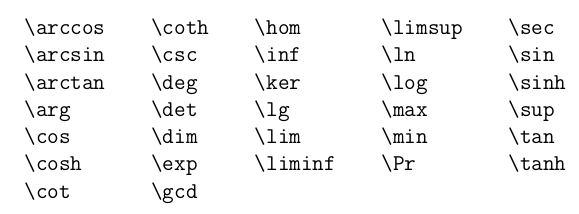
\includegraphics[scale=0.5]{images/math_forms}
	\end{figure}
\end{frame}



\begin{frame}[fragile]{\sc Derivadas}
	\begin{itemize}
		\setlength\itemsep{0.3cm}
   \item Para adicionar {\color{blue} derivadas} ou {\color{blue} derivadas parciais}, escrevemos:
\begin{verbatim}
   \begin{align*}
   \frac{d}{dx}\left[3x^{2}\right]\quad, \quad
   \frac{\partial}{\partial x} \left[3x^{2}+2xy^{3}\right]
   \end{align*}
\end{verbatim}
   e obtemos
   \begin{align*}
   \frac{d}{dx}\left[3x^{2}\right]\quad, \quad
   \frac{\partial}{\partial x} \left[3x^{2}+2xy^{3}\right];
   \end{align*}
   \item Os comandos \verb|\left| e \verb|\right| são utilizados para {\color{blue} ajustar} 
   automaticamente qualquer {\color{blue} delimitador} (\verb|()|, \verb|[]| ou \verb|{}|) 
   ao {\color{blue} tamanho da equação}.
	\end{itemize}
\end{frame}



\begin{frame}[fragile]{\sc Integrais}
	\begin{itemize}
		\setlength\itemsep{0.3cm}
   \item Para adicionar {\color{blue} integrais} e {\color{blue} limites de integração}, utilizamos os comandos 
   \verb|\int\limits{}^{}| ;
   \item Exemplo: Escrevendo \\
\begin{verbatim}
   \begin{align*}
   \int\limits_{x_{0}}^{x}x dx 
   \end{align*}
\end{verbatim}
   obtemos
   \begin{align*}
   \int\limits_{x_{0}}^{x_1}x dx 
   \end{align*}
   \item OBS: não é necessário usar o comando \verb|\limits|. Sem ele o resultado é 
   \begin{align*}
   \int_{x_{0}}^{x_1}x dx.
   \end{align*}   
	\end{itemize}
\end{frame}


\begin{frame}[fragile]{\sc Integrais}
	\begin{itemize}
		\setlength\itemsep{0.3cm}
		\item para aplicação dos {\color{blue} limites de integração} após a integração, use 
\begin{columns}
	\begin{column}{0.4\textwidth}
		\begin{align}
		\int\limits_{x_0}^{x_1} x dx = \frac{x^2}{2}\Big|^{x_1}_{x_0},
		\end{align}
	\end{column}
	%
	\begin{column}{0.6\textwidth}
		\begin{verbatim}
		\begin{align}
		\int\limits_{x_0}^{x_1} x dx = 
		\frac{x^2}{2}\Big|^{x_1}_{x_0},
		\end{align}
		\end{verbatim}
	\end{column}
\end{columns}
		(usar \verb|\left|| não funciona);
        \item {\color{blue} integrais múltiplas indefinidas} são inseridas com 
        os comandos \verb|\iint|, \verb|\iiint|,\verb|\idotsint|.  Respectivamente: 
        \begin{align}
        \iint, \qquad \iiint, \qquad \iiiint, \qquad, \idotsint
        \end{align}
        \item para inserir uma {\color{blue} integral fechada}, use o 
        comando \verb|\oint|, respectivamente 
        \begin{align}
        \oint
        \end{align}
	\end{itemize}
\end{frame}


\begin{frame}[fragile]{\sc Matrizes}
	\begin{itemize}
		\setlength\itemsep{0.3cm}
   \item Para escrever {\color{blue} matrizes}, utilizamos ambientes matriciais;
   \item abaixo, temos alguns comandos para os diferentes {\color{blue} tipos de delimitadores}:
   \begin{itemize}
   	\item \verb|pmatrix| produz (\ );
   	\item \verb|bmatrix| produz [\ ];
   	\item \verb|Bmatrix| produz $\{\ \}$;
   	\item \verb|vmatrix| produz $|\ |$;
   	\item \verb|Vmatrix| produz $||\ ||$
   \end{itemize}
\end{itemize} 
	\begin{columns}
		\begin{column}[t]{0.3\textwidth}
			\begin{verbatim}
			\begin{align*}
			\begin{pmatrix}
			a & b & c\\
			d & e & f\\
			g & h & i
			\end{pmatrix}
			\end{align*}
			\end{verbatim}
		\end{column}
		
		\begin{column}[t]{0.3\textwidth}			
			\begin{align*}
			\begin{pmatrix}
			a & b & c\\
			d & e & f\\
			g & h & i
			\end{pmatrix}
			\end{align*}		
		\end{column}
	\end{columns}

\end{frame}


\begin{frame}[fragile]{\sc Grupos de Equações}
\begin{itemize}
    \setlength\itemsep{0.3cm}
    \item é possível {\color{blue} agrupar equações} das seguintes formas:
\begin{align}
\begin{cases}
	\nabla \cdot{\bf E} =\dfrac{\rho}{\varepsilon_0}\\
	\nabla \cdot {\bf B}=0\\
	\nabla \times {\bf E}=-\dfrac{{\partial} {\bf  B}}{{\partial} t}\\
	\nabla \times {\bf B}=\mu_0 {\bf J}+\mu_0\varepsilon_0 \dfrac{{\partial} {\bf E}}{{\partial} t} 
\end{cases}
\end{align}
{\fontsize{9pt}{10.0}\selectfont
\begin{verbatim}
\begin{align}
\begin{cases}
\nabla \cdot{\bf E} =\dfrac{\rho}{\varepsilon_0}\\
\nabla \cdot {\bf B}=0\\
\nabla \times {\bf E}=-
\dfrac{{\partial} {\bf  B}}{{\partial} t}\\
\nabla \times {\bf B}=\mu_0 {\bf J}+
\mu_0\varepsilon_0 \dfrac{{\partial} {\bf E}}{{\partial} t} 
\end{cases}	
\end{align}
\end{verbatim}
}
\end{itemize}
\end{frame}


\begin{frame}[fragile]{\sc Grupos de Equações}
\begin{itemize}
    \setlength\itemsep{0.3cm}
    \item e
    \begin{numcases}{}
	\nabla \cdot{\bf E} =\dfrac{\rho}{\varepsilon_0}\\
	\nabla \cdot {\bf B}=0\\
	\nabla \times {\bf E}=-\dfrac{{\partial} {\bf  B}}{{\partial} t}\\
	\nabla \times {\bf B}=\mu_0 {\bf J}+\mu_0\varepsilon_0 \dfrac{{\partial} {\bf E}}{{\partial} t} 
    \end{numcases}
{\fontsize{9pt}{10.0}\selectfont
\begin{verbatim}
\begin{numcases}{}
\nabla \cdot{\bf E} =\dfrac{\rho}{\varepsilon_0}\\
\nabla \cdot {\bf B}=0\\
\nabla \times {\bf E}=-
\dfrac{{\partial} {\bf  B}}{{\partial} t}\\
\nabla \times {\bf B}=\mu_0 {\bf J}+
\mu_0\varepsilon_0 \dfrac{{\partial} {\bf E}}{{\partial} t} 
\end{numcases}	
\end{verbatim}
}
\end{itemize}
\end{frame}

\begin{frame}[fragile]{\sc Equações Matriciais}
\begin{itemize}
    \setlength\itemsep{0.3cm}
\item Como exercício, escreva uma equação matricial semelhantre à abaixo:
\begin{align}
\begin{pmatrix}
 x & u\\
 y & v
\end{pmatrix}
=
\begin{pmatrix}
 a & b \\
 c & d
\end{pmatrix}
+
\begin{pmatrix}
 e & f \\
 g & h 
\end{pmatrix}
\end{align}
\item note que matrizes também podem ser utilizadas para agrupar ou 
escrever sistemas de equações;
\end{itemize}
\end{frame}


\begin{frame}[fragile]{\sc Outros operadores e objetos matemáticos}
\begin{itemize}
    \setlength\itemsep{0.3cm}
    \item operadores e objetos matemáticos devem ser inseridos dentro de um ambiente matemático;
    \item na notação usual, vetores são representados com uma seta "$\to$" sobre um caracter. 
    O comando é \verb|$\vec{a}$| e produz $\vv{a}$; 
    \item chapéus \verb|^| são incluídos pelo comando \verb|$\hat{a}$| ou \verb|$\widehat{a}$|: $\widehat{a}$;
    \item o símbolo $\sim$ é inserido com \verb|$\tilde{a}$| ou \verb|$\widetilde{a}$|: $\widetilde{a}$;
\end{itemize}
\end{frame}


\begin{frame}[fragile]{\sc Outros operadores e objetos matemáticos}
Algums exemplos de objetos mais utilizados são listados abaixo. Veja todos eles na ferramenta "Structure"\ do seu compilador.
\begin{table}[h]
    \begin{tabular}{|l|l|} 
%         		\toprule
        \hline
        $\xrightarrow{abc}$ & \verb|$\xrightarrow{r}$|  \\ \hline
        $\underrightarrow{abc}$ & \verb|$\underrightarrow{abc}$| \\ \hline
        $\stackrel{abc}{=}$ & \verb|$\stackrel{abc}{=}$| \\ \hline
        $\ddot{a}$ & \verb|$\ddot{a}$| \\ \hline
        $\longrightarrow$ & \verb|$\longrightarrow$| \\ \hline
        $\Longrightarrow$ & \verb|$\Longrightarrow$| \\ \hline
		$\sim, \simeq, \approx, \approxeq$ & \verb|$\sim, \simeq, \approx, \approxeq$| \\ \hline
        $\leq, \geq, \lesssim, \gg$ & \verb|$\leq, \geq, \lesssim, \gg$| \\ \hline
        $\times, \otimes, \odot, \oplus$ & \verb|$\times, \otimes, \odot, \oplus$| \\ \hline
%         		\midrule
    \end{tabular}
\end{table}
\end{frame}


\begin{frame}[fragile]{\sc Pacote \texttt{physics}}
\begin{itemize}
    \setlength\itemsep{0.3cm}
    \item O pacote {\color{blue}\verb|physics|}, quando incluido no preâmbulo, adiciona comandos convenientes para fácil acesso à símbolos matemáticos usados comumente. Por exemplo:
\begin{table}[h!]
  \centering
  \begin{adjustbox}{max width=\textwidth}
       \begin{tabular}{|l|l|}
        \hline
        $\vb{a}, \va{a}, \vu{a}$ & \verb|$\vb{a}, \va{a}, \vu{a}$|\\ %& Negrito, seta e unitário. Sem letra grega. \\
        \hline
        $\vb*{a}, \va*{a}, \vu*{a}$& \verb|$\vb*{a}, \va*{a}, \vu*{a}$|\\% & Negrito, seta e unitário. Itálco e com letra grega\\
        \hline
        $\vdot, \cross, \cp$ & \verb|$\vdot, \cross, \cp$|\\%& Produto escalar e vetorial\\
        \hline
        $\div, \grad, \curl, \laplacian$ & \verb|$\div, \grad, \curl, \laplacian$|\\% & Divergente, Gradiente, Rotacional e Laplaciano\\
        \hline
        $\dd{x}, \dv{x}, \pdv{x}$ & \verb|$\dd{x}, \dv{x}, \pdv{x}$|\\ %& Diferencial, Derivada e Derivada Parcial\\
        \hline
        $\dd[n]{x}, \dv[n]{f}{x}, \pdv[n]{f}{x}$ & \verb|$\dd[n]{x}, \dv[n]{f}{x}, \pdv[n]{f}{x}$|\\ %& Diferencial, Derivada e Derivada Parcial de ordem n.\\
        \hline
         $\ket{x}, \bra{x}$ & \verb|$\ket{x}, \bra{x}$|\\ %& Notação Bracket\\
        \hline
         $\braket{a}{b}, \op{a}{b}$ & \verb|$\braket{a}{b}, \op{a}{b}$| \\%& Produto Interno e Externo\\
        \hline
             $\expval{a}, \ev{a}{\Psi}, \mel{n}{a}{m}$ & \verb|$\expval{a}, \ev{a}{\Psi}, \mel{n}{a}{m}$|\\ %& Valor esperado e elemento de matriz\\
        \hline
        \end{tabular}
        \end{adjustbox}
\end{table}
\end{itemize}
\end{frame}

\begin{frame}[fragile]{\sc Estilizando fontes}
É muito comum, em muitas vezes, ocorrer {\color{blue} carência de símbolos} matemáticos. 
Para isso, é possível modificar o {\color{blue} estilo da fonte} 
das letras do alfabeto latino dentro do ambiente matemático. Alguns exemplos são:\\[0.5cm]
\verb|\mathbf{AaBbCc}| texto negrito $\mathbf{AaBbCc}$\\
\verb|\mathit{AaBbCc}| texto itálico $\mathit{AaBbCc}$\\
\verb|\mathrm{AaBbCc}| texto padão $\mathrm{AaBbCc}$\\
%\verb|\mathttt{AaBbCc}| texto ``terminal'' $\mathttt{AaBbCc}$\\
%\verb|\mathsf{AaBbCc}| texto negrito ``sanserif'' $\mathsf{AaBbCc}$\\
\verb|\mathcal{ABC}| texto caligráfico $\mathcal{ABC}$\\
\verb|\mathbb{ABC}| texto em lousa $\mathbb{ABC}$, requer \verb|amssymb| \\
\verb|\mathscr{ABC}| texto estilizado $\mathscr{ABC}$, requer \verb|mathrsfs|;\\
\verb|\mathfrak{AaBbCc}| texto $\mathfrak{AaBbCc}$;
%		\begin{figure}[h]
%			\centering
%			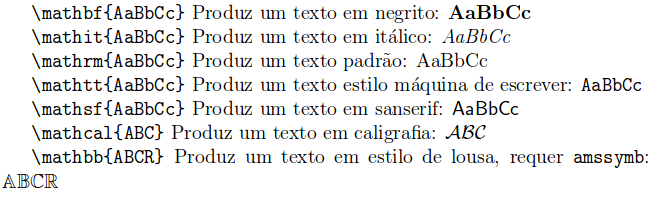
\includegraphics[scale=0.43]{images/fontes.png}
%		\end{figure}

\end{frame}	


\section{Tabelas}
\subsection{Criando Tabelas}
\plain{Criando Tabelas.}

\begin{frame}[fragile]{\sc Tabelas}
	\begin{itemize}
		\setlength\itemsep{0.3cm}
		\item Uma {\color{blue} tabela} é especificada pelo ambiente {\color{blue} \verb|tabular|};
%		\item a criação de tabelas é relativamente simples, entretanto em alguns casos pode gerar transtornos;
		\item a criação de uma tabela é feita da seguinte forma:
		\verb| \begin{tabular}{espec} |\\
		em que o argumento {\color{blue} \verb|espec|} especifica a {\color{blue} quantidade de colunas} e o seu {\color{blue} alinhamento}:    
		\begin{itemize}
			\item $|$ adiciona uma linha vertical;
			\item \verb|l| indica uma coluna alinhada à esquerda;
			\item \verb|r| indica uma coluna alinhada à direita;
			\item \verb|c| indica uma coluna com texto centralizado;
		\end{itemize} 
		\item Quanto ao {\color{blue} preenchimento da tabela}, utilizamos:
		\begin{itemize}
			\item \verb|&| para passar para a próxima coluna;
			\item \verb| \\ | para terminar uma linha e criar para uma nova;
			\item \verb|\hline| para criar uma linha horizontal.
		\end{itemize} 
	\end{itemize}
\end{frame}



\begin{frame}[fragile]{\sc Tabelas}
	\begin{itemize}
		\setlength\itemsep{0.3cm}
		\item uma tabela pode ser inserida dentro do {\color{blue} ambiente \verb|table|}, o que faz dela
		um {\color{blue} objeto flutuante};
		\item {\color{blue} vantagens} de utilizar esse tipo de ambiente:
		\begin{itemize}
			\item posição correta da tabela no texto;
			\item permite a inserção de rótulos e legendas;
			\item faz com que a tabela apareça em um índice de tabelas;
		\end{itemize}
		\item Para usar este ambiente é preciso usar o comando\\ 
		\verb|\begin{table}[pos]|\\
		em que {\color{blue} \verb|pos|} indica a posição desejada para se {\color{blue} posicionar a tabela verticalmente} na página: 
		\begin{itemize}
			\item \textbf{h} no local onde o texto ocorreu;
			\item \textbf{t} no topo da página;
			\item \textbf{b} no fim da página;
			\item \textbf{p} em uma página especial contendo somente objetos flutuantes;
		\end{itemize}
	\end{itemize}
\end{frame}
%
\begin{frame}[fragile]{\sc Tabelas}
	\begin{itemize}
				\setlength\itemsep{0.3cm}
		\item Para {\color{blue} adicionar uma legenda} usamos, ainda dentro do ambiente \verb|table|, o comando\\
		\verb|\caption{legenda}|
		\item A seguir apresentamos uma tabela criada como objeto flutuante e os comandos utilizados para que fosse gerada:
	\end{itemize}
\end{frame}

\begin{frame}[fragile]{\sc Tabelas}
	\begin{table}[h]
		\begin{tabular}{c|c} 
			\toprule
			\textbf{RS}             &\textbf{Temperatura Máxima} ($^{\circ}C)$\\
			\midrule
			Porto Alegre             &39\\ \hline
			Santa Maria              &40\\ \hline
			Rio Grande               &40\\ \hline
			Pelotas                  &40\\ \hline
			Caxias do Sul            &38\\ \hline 
			\bottomrule
		\end{tabular}
	\end{table}
\end{frame}

\begin{frame}[fragile]{\sc Tabelas}
	\centering
	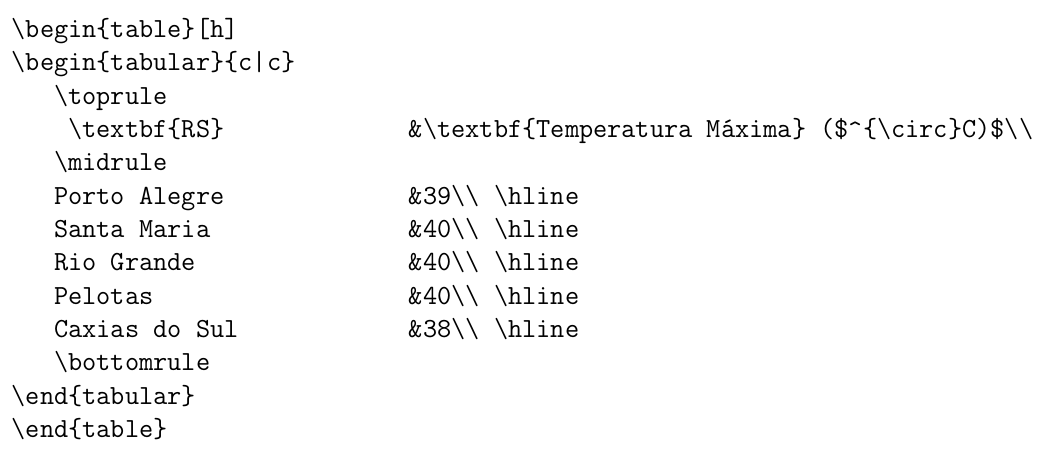
\includegraphics[scale=0.3]{images/exemplo_tabela.png}
\end{frame}
%
\begin{frame}[fragile]{\sc Exemplos de Tabelas}
\begin{table}[h]
\begin{tabular}{c|c|c|c} 
				\toprule
				\textbf{Qualidade da construção}       &\textbf{a}                       &\textbf{b}                     &\textbf{c}\\
				\midrule
				Boa vedação                   &0,15                    &0,010                 &0,007\\
				Média                         &0,20                    &0,015                 &0,014\\
				Má vedação                    &0,25                    &0,020                 &0,022\\
				\bottomrule 
\end{tabular}
\end{table}
		
\begin{table}[h]
\begin{tabular}{c|c|c} 
				\toprule
				\textbf{Resistência}              &\textbf{Expressão}                                                       &\textbf{Efeito}                \\
				\midrule
				\multirow{2}{*}{$R_{1}$}           &\multirow{2}{*}{$\displaystyle\frac{1}{h_{i}2\pi r_{1}L}$}               &\multirow{2}{*}{Inalterada}    \\ 
				&                                                                         &                               \\ \hline 
				\multirow{2}{*}{$R_{2}$}           &\multirow{2}{*}{$\displaystyle\frac{\ln(r_{2}/r_{1})}{K_{t}2\pi L}$}     &\multirow{2}{*}{Inalterada}    \\ 
				&                                                                         &                               \\ \hline
				\multirow{2}{*}{$R_{3}$}           &\multirow{2}{*}{$\displaystyle\frac{\ln(r_{3}/r_{2})}{K_{iso}2\pi L}$}   &\multirow{2}{*}{Aumenta}       \\ 
				&                                                                         &                               \\ \hline
				\multirow{2}{*}{$R_{4}$}           &\multirow{2}{*}{$\displaystyle\frac{1}{h_{e}2\pi r_{3}L}$}               &\multirow{2}{*}{Diminui}       \\ 
				&                                                                         &                               \\ \hline
				\bottomrule
				%NÃO PRECISAVA DE TODA ESSA COMPLICAÇÃO ACIMA PARA FAzER A TABELA!!!
\end{tabular}
\end{table}
\end{frame}
	
	\begin{frame}
		\frametitle{\sc Exemplo de Tabelas}
		\begin{table}[c]
			\begin{center}
				\resizebox{10cm}{!}{\begin{tabular}{c|c|c|c|c|c} 
						\toprule
						\multirow{2}{*}{\textbf{Material Isolante}}             &\multirow{2}{*}{$Kgf/m^{3}$}        &\multirow{2}{*}{$k\frac{Kcal}{mh^{\circ}C}$}     &\textbf{Resistência}                         &\textbf{Resistência à}                           &\textbf{Permeabilidade}      \\
						&                                    &                                                 &\textbf{Mecânica:}$Kgf/m^{2}$                &\textbf{temperatura:}$^{\circ}C$                 &$g/m.h.mmHg$            \\
						\midrule
						Aço ordinário                                            &7800                                &45 a 50                                          &                                    &                                        &Nula\\ \hline
						Vidro                                                    &2500                                &0,65                                             &                                    &                                        &Nula\\ \hline
						Concreto                                                 &2300                                &1,2                                              &                                    &                                        &22,3\\ \hline
						Pedra (granito)                                          &2600                                &3                                                &                                    &                                        &\\ \hline
						Alvenaria                                                &1800                                &0,84                                             &                                    &                                        &220,98\\ \hline
						Asfalto                                                  &2120                                &0,65                                             &                                    &                                        &\\ \hline
						Madeira (pinho)                                          &550                                 &0,14 a 0,3                                       &                                    &                                        &6,0 a 9,0\\ \hline
						Serragem de madeira                                      &200                                 &0,06                                             &                                    &                                        &\\ \hline
						Fibra de madeira aglomerada                              &\multirow{2}{*}{210}                &\multirow{2}{*}{0,028}                           &\multirow{2}{*}{20}                 &                                        &\multirow{2}{*}{30 a 2800}\\
						(Eucatex frigorífico)                                    &                                    &                                                 &                                    &                                        &\\ \hline 
						Cortiça                                                  &200                                 &0,045                                            &1                                   &100                                        &66\\ \hline
						Cortiça aglomerada                                       &200                                 &0,036                                            &                                    &100                                     &\\ \hline
						Lã de vidro                                              &100 a 200                           &0,025 a 0,045                                    &                                    &540                                     &80\\ \hline
						Lã de rocha                                              &100 a 200                           &0,025 a 0,035                                    &                                    &600                                     &\\ \hline
						Vermiculite (cortiça mineral)                            &70                                  &0,04                                             &Fraca                               &1000                                    &10 a 39\\ \hline
						Concreto celular                                         &300 a 600                           &0,049 a 0,12                                     &                                    &                                        &\\ \hline
						Espuma de plástico                                       &25                                  &0,035                                            &                                    &80                                      &\\ \hline
						Espuma de borracha                                       &80                                  &0,03                                             &                                    &65                                      &\\ \hline
						Poliestireno expandido                                   &\multirow{2}{*}{15 a 30}            &\multirow{2}{*}{0,028}                           &\multirow{2}{*}{0,3 a 0,7}          &                                        &\multirow{2}{*}{1,3 a 1,82}\\
						(styropor)                                               &                                    &                                                 &                                    &                                        &\\ \hline 
						Espuma fanólica rígida                                   &30 a 45                             &0,026                                            &Fraca                               &                                        &\\ \hline
						Espuma rígida de Poliestireno                            &\multirow{2}{*}{30}                 &\multirow{2}{*}{0,028}                           &\multirow{2}{*}{1,0 a 2,0}          &                                        &\\
						(styrofoan)                                              &                                    &                                                 &                                    &                                        &\\ \hline
						Espuma rígida de poliuretano                             &\multirow{2}{*}{30 a 45}            &\multirow{2}{*}{0,02}                            &\multirow{2}{*}{2}                  &                                        &\multirow{2}{*}{Baixa}\\
						(moltopren)                                              &                                    &                                                 &                                    &                                        &\\ \hline
						Espuma rígida de vidro                                   &\multirow{2}{*}{145}                &\multirow{2}{*}{0,046}                           &\multirow{2}{*}{7}                  &\multirow{2}{*}{430}                    &\multirow{2}{*}{Nula}\\
						(foamglass)                                              &                                    &                                                 &                                    &                                        &\\ \hline
						\bottomrule
					\end{tabular}}
				\end{center}
			\end{table}
		\end{frame}    
%		


\section{Figuras}
\subsection{Inserindo Figuras}
\plain{Vamos agora trabalhar com figuras.}
\begin{frame}[fragile]{\sc Inserindo Figuras}	
\begin{itemize}
			\setlength\itemsep{0.3cm}
	\item Para {\color{blue} acrescentar figuras} nos documentos, será necessária a declaração de um {\color{blue} novo pacote}
    \begin{verbatim}
    \usepackage{graphicx}
    \end{verbatim}
    \item Assim, podemos incluir figuras com o seguinte comando no corpo do texto
    \begin{verbatim}
        \includegraphics[opt]{nomedafigura}
    \end{verbatim}
    \item Como \verb|opt| podemos passar as seguintes opções:
    \begin{itemize}
        \item \verb|width|: Redimensiona a figura para a largura especificada;
        \item \verb|heigth|: Redimensiona a figura para a altura especificada;
        \item \verb|angle|: Rotaciona a figura no sentido horário (em graus);
        \item \verb|scale|: Redimensiona a figura na proporção especificada.
    \end{itemize} 

\end{itemize}
\end{frame}

		
\begin{frame}[fragile]{\sc Inserindo Figuras}
	\begin{itemize}
				\setlength\itemsep{0.3cm}
		\item Existe um {\color{blue} ambiente específico} para tratar uma {\color{blue} figura} como um {\color{blue} objeto flutuante} chamado \verb| figure |, e permite inserir legendas; 
		\item a seguir, apresentamos um exemplo\\
		\begin{verbatim}
		\begin{figure}[h]
		\centering
		\includegraphics[width=0.99\linewidth]{nomedafigura}
		\caption{Uma figura qualquer}
		\label{label_da_figura}
		\end{figure}
		\end{verbatim}
		\item as opções do ambiente figura são os mesmos que das tabelas;
		\item em adicional, muitas vezes a opção h não faz o que gostaríamos. Se isso ocorrer, use H 		e o \LaTeX\  irá colocar a figura exatamente onde ela é inserida no texto;
		\item OBS: use isso em últimos casos;
	\end{itemize}
\end{frame}
		
\begin{frame}[fragile]{\sc Inserindo Figuras}
			\begin{figure}[h]
				\centering
				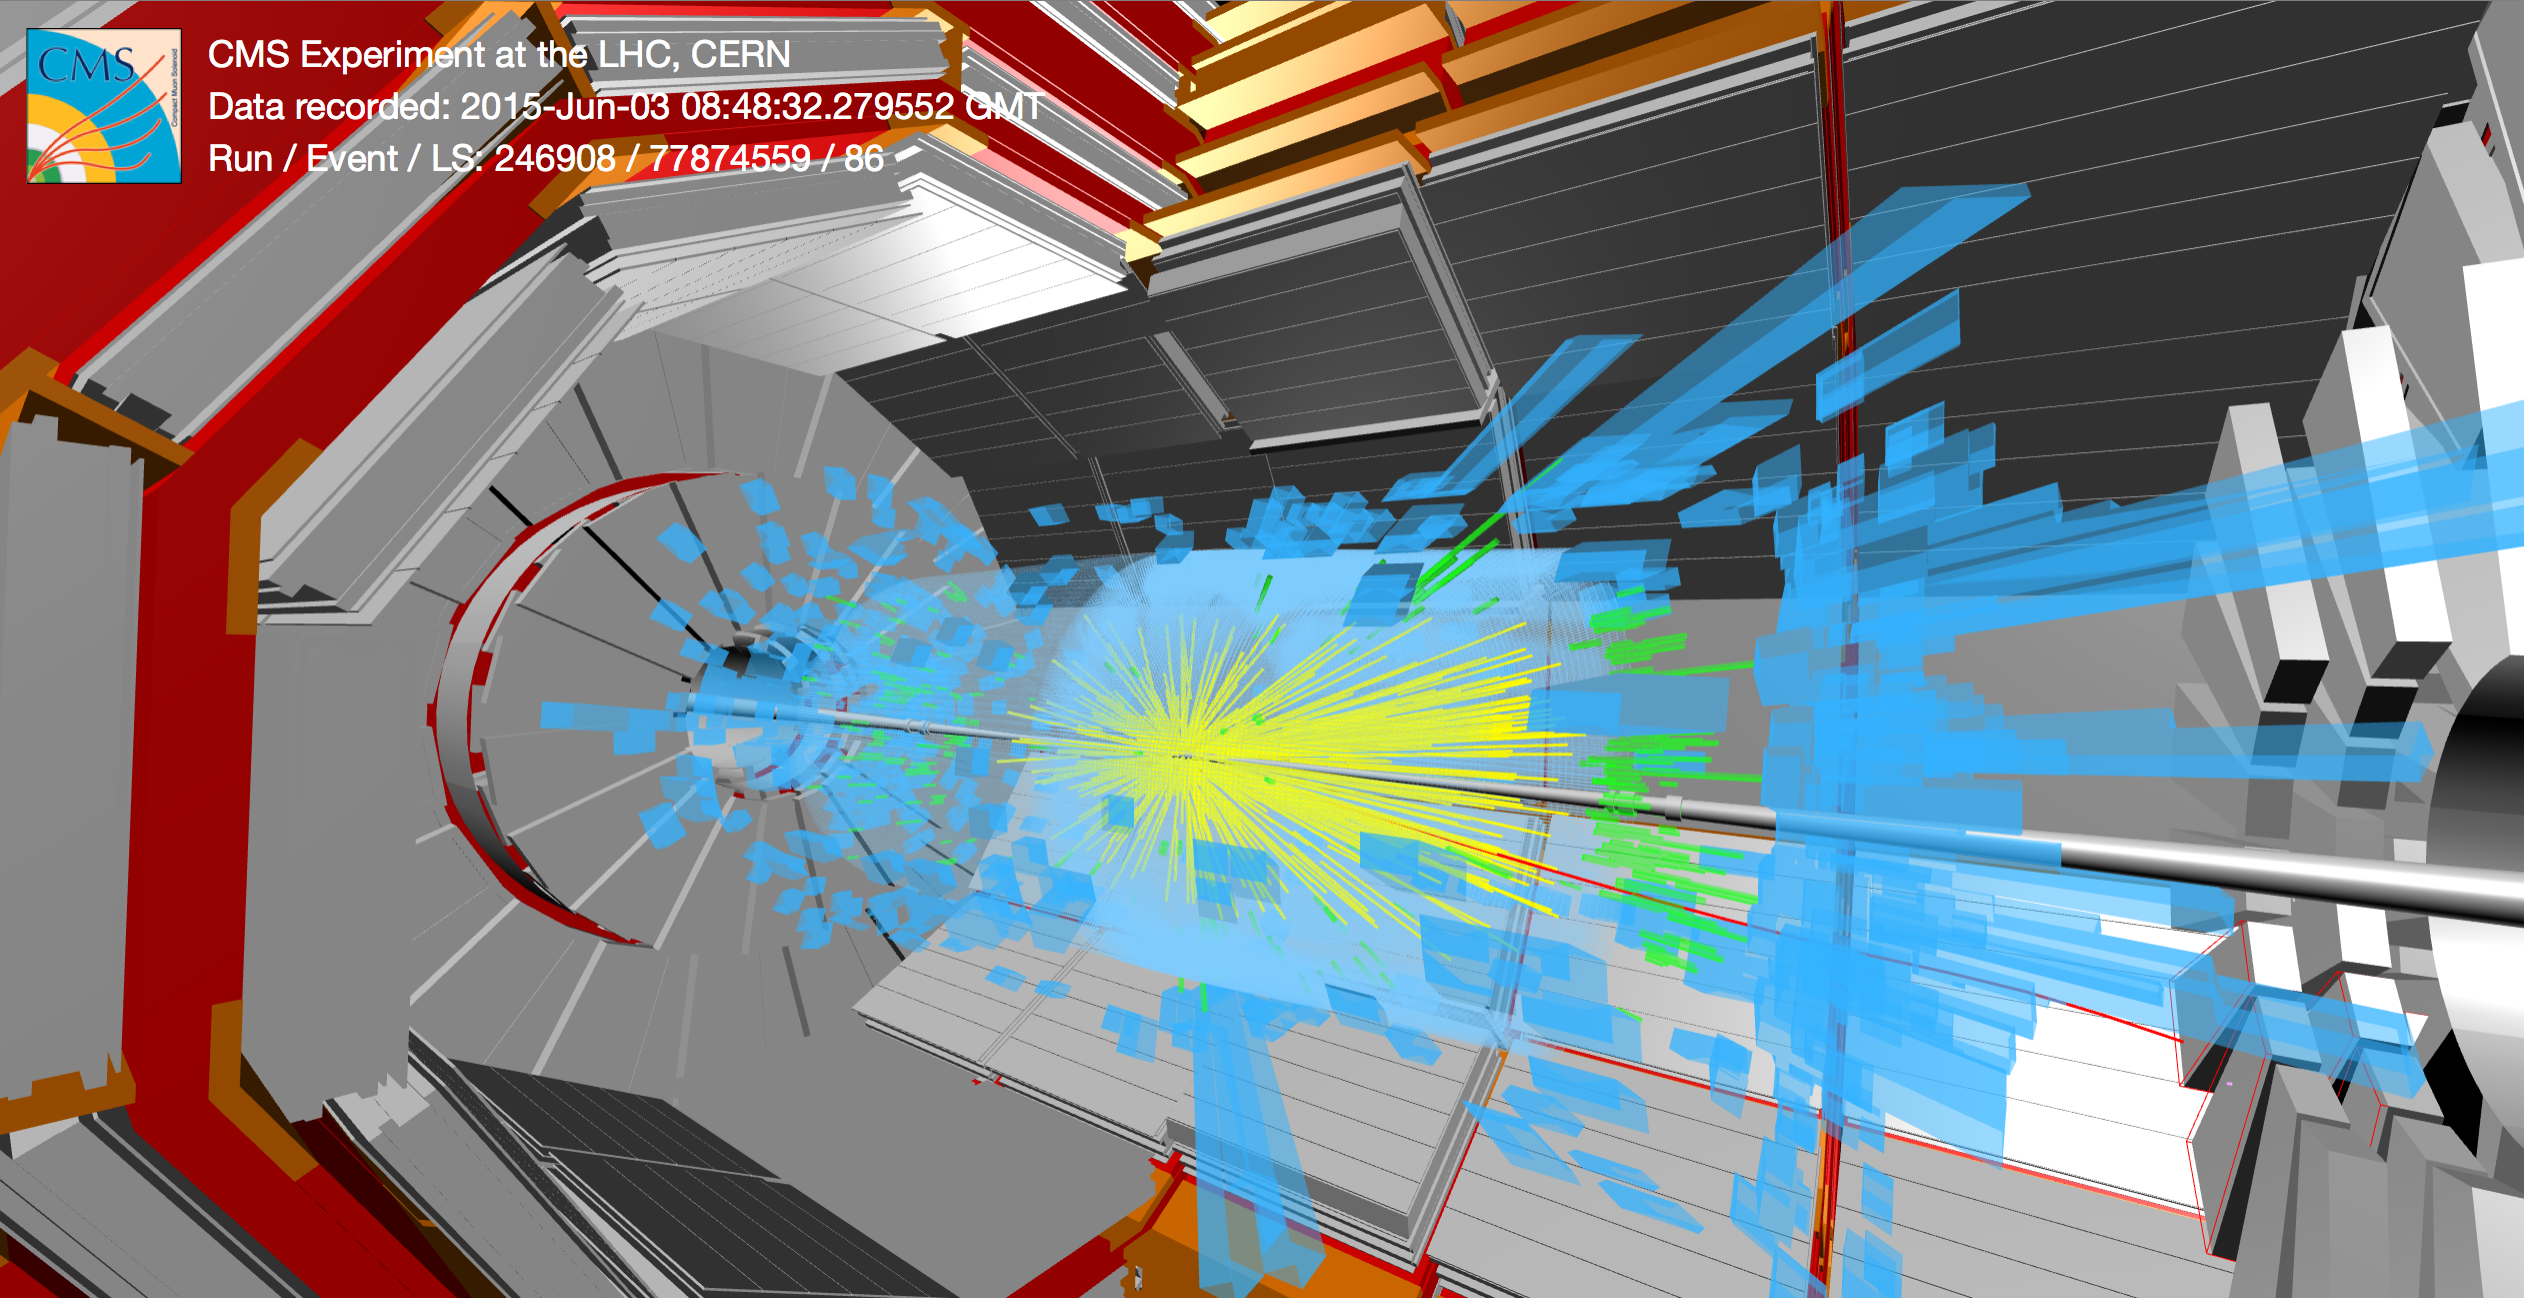
\includegraphics[width=0.99\linewidth]{images/exemplo_de_figura}
				\caption{Uma figura qualquer}
			\end{figure}
\end{frame}

\begin{frame}[fragile]{Inserindo mais de uma figura}
			
			Podemos adicionar mais de uma figura no mesmo ambiente ao utilizar o comando \verb|\includegraphics[tamanho]{nomedafigura}|. Porém, temos que ter cuidado com os tamanhos das figuras e as posições.
			\begin{itemize}
						\setlength\itemsep{0.3cm}
				\item Figura lado a lado: incluir os comandos \verb|\includegraphics[]{}| um em baixo do outro
				\item Figura em cima e embaixo: incluir os comandos \verb|\includegraphics[]{}| separados por \verb| \\ |
			\end{itemize}
			
\end{frame}
		
\begin{frame}[fragile]{\sc Exemplo - Figura lado a lado}
\begin{verbatim}
			\begin{figure}[h]
			\centering
			
\includegraphics[scale=0.15]{images/furg.png}
			
\includegraphics[scale=0.1]{images/imef2.png}
			\caption{Exemplo:lado a lado}
			\end{figure}
\end{verbatim}
			\begin{figure}[H]
				\centering
				
\includegraphics[scale=0.15]{images/furg.png}
				
\includegraphics[scale=0.1]{images/imef2.png}
				\caption{Exemplo:lado a lado}
			\end{figure}
\end{frame}
		
		
\begin{frame}[fragile]{\sc Exemplo - Figura em cima e embaixo}
			\begin{columns}
				\begin{column}{0.5\textwidth}
					\scriptsize
\begin{verbatim}
					\begin{figure}[h]
					\centering
					
\includegraphics[scale=0.15]{images/furg.png} \\
					
\includegraphics[scale=0.1]{images/imef2.png}
					\caption{Exemplo: em cima e embaixo}
					\end{figure}
\end{verbatim}					
				\end{column}
				
				\begin{column}{0.5\textwidth}
					\begin{figure}
						\centering
						
\includegraphics[scale=0.15]{images/furg.png} \\
						
\includegraphics[scale=0.1]{images/imef2.png}
						\caption{Exemplo: em cima e embaixo}
					\end{figure}
				\end{column}
			\end{columns}
\end{frame}
				
\begin{frame}[fragile]{\sc Inserindo figuras com subtítulos}
			Para ter um controle de {\color{blue} títulos e subtítulos de figuras} devemos utilizar o ambiente {\color{blue}\verb|subfigure|} e o pacote \verb|subcaption| no preambulo.
\begin{figure}[h]
				\centering
\begin{subfigure}{0.5\textwidth}
					\centering
					
\includegraphics[scale=0.1]{images/furg.png}
					\caption{FURG}
\end{subfigure}%
\begin{subfigure}{0.5\textwidth}
					\centering
					
\includegraphics[scale=0.1]{images/imef2.png}
					\caption{IMEF}
\end{subfigure}
				\caption{Exemplo de figuras com subtítulos}
\end{figure}
			
\end{frame}
		
\begin{frame}[fragile]{\sc Inserindo figuras com subtítulos - Código}
			\scriptsize
			\begin{verbatim}
  \begin{figure}[h]
    \centering
  \begin{subfigure}{0.5\textwidth}
        \centering
        
\includegraphics[scale=0.1]{images/furg.png}
        \caption{FURG}
  \end{subfigure}%
  \begin{subfigure}{0.5\textwidth}
        \centering
        
\includegraphics[scale=0.1]{images/imef2.png}
        \caption{IMEF}
  \end{subfigure}
    \caption{Exemplo de figuras com subtítulos}
  \end{figure}
			\end{verbatim}
\end{frame}

\section{Referenciando objetos}

\plain{Referenciando figuras, tabelas e equações ao longo do texto.}


\begin{frame}[fragile]{\sc Lidando com referências}
	Uma das grandes vantagens do \LaTeX \ é a facilidade de fazer {\color{blue} referências} a figuras, tabelas, equações, artigos, livros, etc.. 
	\\
	Para {\color{blue} citar} alguma {\color{blue} figura}, {\color{blue} tabela} ou {\color{blue} equação}, devemos adicionar o comando,
	\begin{verbatim}
		\label{nome}
	\end{verbatim}
	em que \texttt{nome} será utilizado para a citação.
	\\
	Para chamar no texto, devemos utilizar o comando, 
	\begin{verbatim}
		\ref{nome}
	\end{verbatim}
	
\end{frame}

\begin{frame}{\sc Lidando com referências - Exemplo}	
	\begin{equation}
	\nabla \cdot \vv{E} = \frac{Q}{\varepsilon_0} \label{maxwell}
	\end{equation}	
	\begin{figure}[h]
		\centering
		
\includegraphics[scale=0.05]{images/furg.png}
		\caption{Logo FURG}
		\label{furg}
	\end{figure}
	A equação (\ref{maxwell}) é a primeira equação de Maxwell. A {\sc Figura} \ref{furg} é o logo da FURG.
\end{frame}

\begin{frame}[fragile]{\sc Lidando com referências - Código do Exemplo}
	\scriptsize
	\begin{verbatim}
	\begin{equation}
	\nabla \cdot \vec{E} = \frac{Q}{\varepsilon_0} \label{maxwell}
	\end{equation}

	\begin{figure}[h]
	\centering
	
\includegraphics[scale=0.05]{furg.png}
	\caption{Logo FURG}
	\label{furg}
	\end{figure}
	
	A equação (\ref{maxwell}) é a primeira equação de Maxwell.
	A {\sc Figura} \ref{furg} é o logo da FURG.
	\end{verbatim}
\end{frame}

\begin{frame}[fragile]{\sc O pacote \texttt{cleveref}}
\begin{itemize}
\item Com o pacote {\color{blue}\verb|cleveref|} é possível referenciar {\color{blue} multiplos objetos} ao mesmo tempo. Por exemplo usando o código:
\begin{verbatim}

\begin{align}
a = b + c \label{a} \\ 
c = d + e \label{b} \\ 
e = f + g \label{c} \\ 
g = h + j \label{d}
\end{align}

As \cref{a,b,c,d} são do tipo recorrente.
\end{verbatim}

\item Obtemos :
\begin{align}
a = b + c \label{f1}\\ 
c = d + e \label{f2}\\ 
e = f + g \label{f3}\\ 
g = h + j  \label{f4}
\end{align}

As \cref{f1,f2,f3,f4} são do tipo recorrente.

\end{itemize}
\end{frame}

\begin{frame}[fragile]{\sc O pacote \texttt{cleveref}}
\begin{itemize}
\item Note que o pacote automaticamente adiciona {\color{blue} eqs.}, os numeros das equações {\color{blue} inicial} e {\color{blue}final} referenciadas além da conjunção {\color{blue} to}. A linguagem padrão do pacote é inglês.
\item Para modificar as conjunções para português, basta renovar os comandos no preâmbulo:
\begin{verbatim}
\newcommand{\crefrangeconjunction}{} 
%Para varias referências (ex: eqs. 5 à 10)
\newcommand{\crefmiddleconjunction}{} 
%Para equações não consecutivas (ex:eqs 3, 5 e 10)
\newcommand{\crefpairconjunction}{}
%Para pares de referências (ex:eqs. 3 e 4) 
\end{verbatim}
Com a conjunção desejada entre parênteses. 

\end{itemize}
\end{frame}

% \section{Apresentações Beamer}


% {\fontsize{10pt}{10.0}\selectfont

\section{Apresentações Beamer}
\subsection{Estrutura}
\plain{Como criar apresentações de slides utilizando o \LaTeX?}
\plain{Através da classe \texttt{beamer} !}

\begin{frame}[fragile]{{\sc Estrutura do }\texttt{beamer}}
	\begin{itemize}
		\setlength\itemsep{0.3cm}
  \item Em \LaTeX\ é possível criar apresentações de uma forma simples e de qualidade, com o pacote \verb| beamer |. Basta definir como classe:\\
  \begin{verbatim}
	\documentclass[opções]{beamer}
  \end{verbatim}
  \item algumas opções são tamanho \verb|8pt,9pt,10pt,11pt,...|;
  \item o uso de pacotes é idêntico às outras classes \verb| book, article | etc.;
  \item informações básicas sobre o documento são:\\
\begin{verbatim}
  \title{}
  \subtitle{}
  \date[]{}
  \author{}
  \institute{}
  \logo{}
  \end{verbatim}
	\end{itemize}
\end{frame}



\begin{frame}[fragile]{{\sc Estrutura do }\texttt{beamer}}
	\begin{itemize}
		\setlength\itemsep{0.3cm}
		\item da mesma forma que outras classes, tudo o que estiver entre 
		\begin{center}
			\verb| \begin{document} |\\
			.\\
			.\\
			.\\
			\verb| \end{document} |
		\end{center}
		constitui-rá tudo o que estiver escrito nos \emph{frames}: textos, listas, tabelas, figuras, equações etc;
		\item um frame é uma página da apresentação, e é construído por:\\
		\verb|\begin{frame}[opções]{título}{subtítulo}|\\
		\verb|\end{frame}|
		\item exemplo de opções: 
		\begin{itemize}
			\item  \verb|fragile|, usado para \emph{macros}, como o \verb|verbatim|;\\
			\item \verb|b|, \verb|c| ou \verb|t|, posição do texto no frame (\verb|b| este frame);
		\end{itemize}
	\end{itemize}
\end{frame}






\begin{frame}[fragile]{{\sc Estrutura do }\texttt{beamer}}
	\begin{itemize}
		\setlength\itemsep{0.3cm}
		\item para se criar o sumário da apresentação, crie um frame e insira o comando \verb|\tableofcontents| da seguinte forma:
        \begin{verbatim}
		    \begin{frame}{Sumário}
		    \tableofcontents
		    \end{frame}|
        \end{verbatim}
		\item se caso o sumário for muito grande e não couber no frame, crie duas colunas (a seguir) ou use o comando 
		\verb|{\fontsize{10pt}{10.0}\selectfont frame do sumário aqui }|;
	\end{itemize}
\end{frame}

\subsection{Ambientes do \texttt{beamer}}
\plain{Vejamos agora alguns ambientes utilizados no \texttt{beamer}}

\begin{frame}[fragile]{{\sc Blocos}}
	\begin{itemize}
		\setlength\itemsep{0.3cm}
		\item ambientes muito utilizados nos beamers são: \verb|itemize|, \verb|enumerate|, \verb|description|;
		\item outros ambientes são os \verb|blocos|: \verb|block|, \verb|alertblock|, \verb|exampleblock|, ...
	\end{itemize}
\begin{figure}[h]
	\centering
	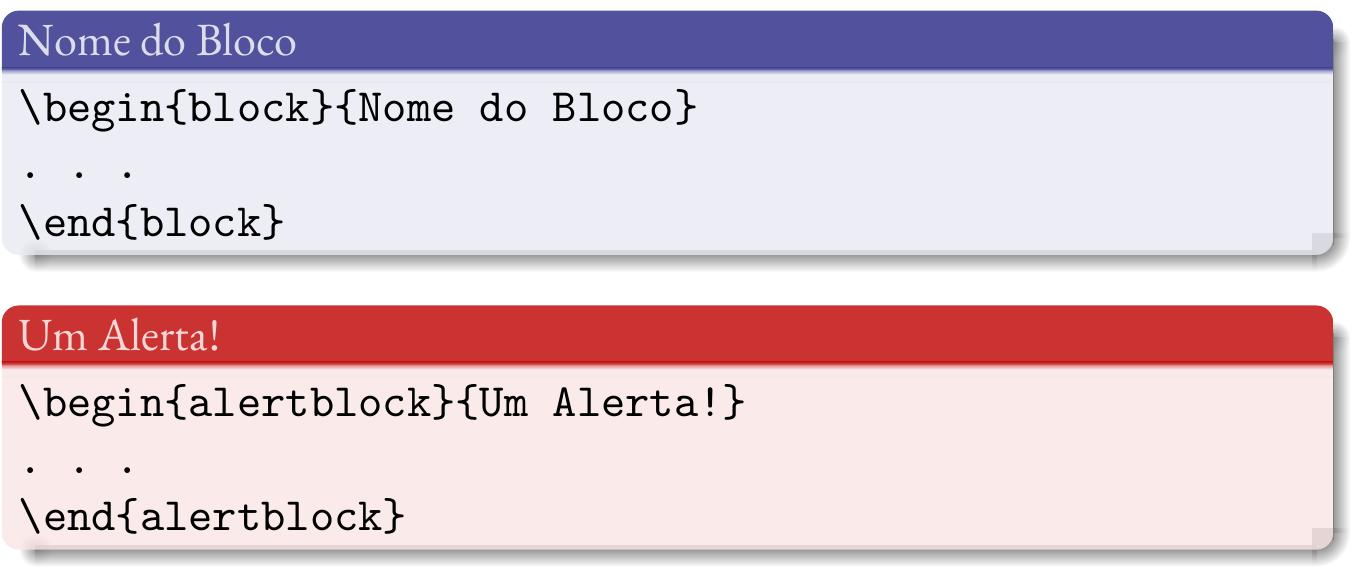
\includegraphics[width=0.99\textwidth]{images/blocks_1.jpg}
\end{figure}
\end{frame}




\begin{frame}[fragile]{\sc Colunas}
	\begin{itemize}
		\setlength\itemsep{0.3cm}
		\item dividir um frame em colunas pode ser bastante útil;
		\item para criá-las basta usar:
		%
		\begin{columns}
			\begin{column}{5cm}
				
				\begin{verbatim}
				\begin{columns}
				\begin{column}[t]{tamanho}
				Criando colunas.
				Duas colunas.
				\end{column}
				\end{verbatim}
				
			\end{column}
			
			\begin{column}{5cm}
				
				\begin{verbatim}     
				\begin{column}[t]{tamanho}
				Tamanho define a largura 
				das colunas. 
				\end{column}
				\end{columns}
				\end{verbatim}
				
			\end{column}
			
		\end{columns}
		\item em uma coluna podemos ter um texto e na outra uma figura (exercício).
	\end{itemize}
\end{frame}

\begin{frame}[fragile]{\sc Colunas - Exercício}
	\begin{columns}
		
		\begin{column}[t]{6cm}
			\begin{figure}[b]
				\centering
				\includegraphics[scale=0.18]{images/NGC_5371.jpg}
				\caption{NGC 5371 - Galáxia espiral barrada, localizada a $\sim$ 100 milhões de anos luz da Terra, 
					na constelação de  Canes Venatici.}
				\label{mod_3_ex_1}
			\end{figure}
			
		\end{column}
		
		
		\begin{column}[t]{6cm}
\begin{figure}[h]
	\centering
	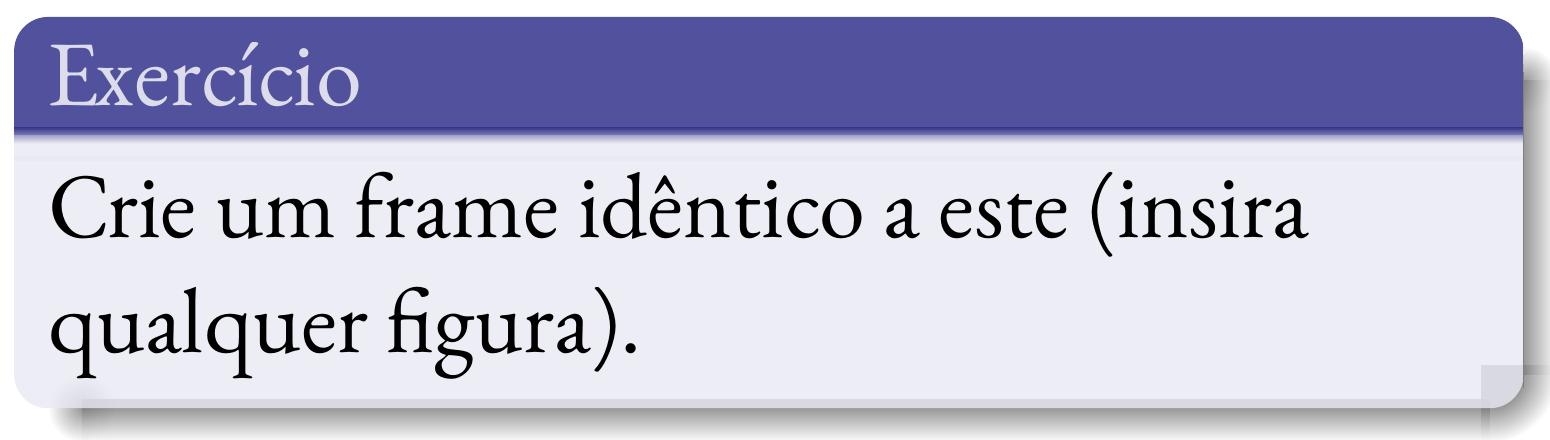
\includegraphics[width=0.99\textwidth]{images/blocks_2.jpg}
\end{figure}
			
			\begin{itemize}
				\item crie duas colunas com 6cm cada;
				\item insira uma figura na coluna esquerda; 
				\item crie um bloco;
				\item faça uma lista qualquer;
			\end{itemize}
			
		\end{column}
		
	\end{columns}
	
\end{frame}


{\fontsize{8pt}{7.0}\selectfont
\begin{frame}[fragile]{\sc Colunas - Exercício}
\begin{verbatim}
\begin{columns}

\begin{column}[t]{6cm}
\begin{figure}[b]
\centering
\includegraphics[scale=0.18]{NGC_5371.jpg}
\caption{NGC 5371 - Galáxia espiral barrada, 
localizada a $\sim$ 100 milhões de anos luz da Terra, 
na constelação de  Canes Venatici.}
\label{mod_3_ex_1}
\end{figure}
\end{column}

\begin{column}[t]{6cm}
\begin{block}{Exercício}
Crie um frame idêntico a este (insira qualquer figura).
\end{block}
\begin{itemize}
\item crie duas colunas com 6cm cada;
\item insira uma figura na coluna esquerda; 
\item crie um bloco;
\item faça uma lista qualquer;
\end{itemize}
\end{column}

\end{columns}
\end{verbatim}
\end{frame}
}


\begin{frame}[fragile]{Temas}
	\begin{itemize}
		\setlength\itemsep{0.3cm}
		\item vários modelos de \emph{beamers} estão disponíveis para utilização;
		\item para isso, modificamos o tema com:\\
		\verb|\usetheme{}| - modifica a estrutura do tema;\\
		\verb|\usecolortheme{}| - modifica a cor do tema;\\
		\verb|\usefonttheme{}| - modifica a fonte do tema
		\item exemplos destes temas são: \verb|\usetheme{Darmstadt}|, \verb|\usecolortheme{orchid}|, \verb|\usefonttheme{serif}|;
		%   \item outras modificações são como a utilizada no exercício, \verb|\setbeamercovered{transparent}|, que deixa também objetos transparentes aos logos nesta 
		%   apresentação;
	\end{itemize}
\end{frame}



\begin{frame}[fragile]{\sc Temas}
\begin{figure}[h]
	\centering
	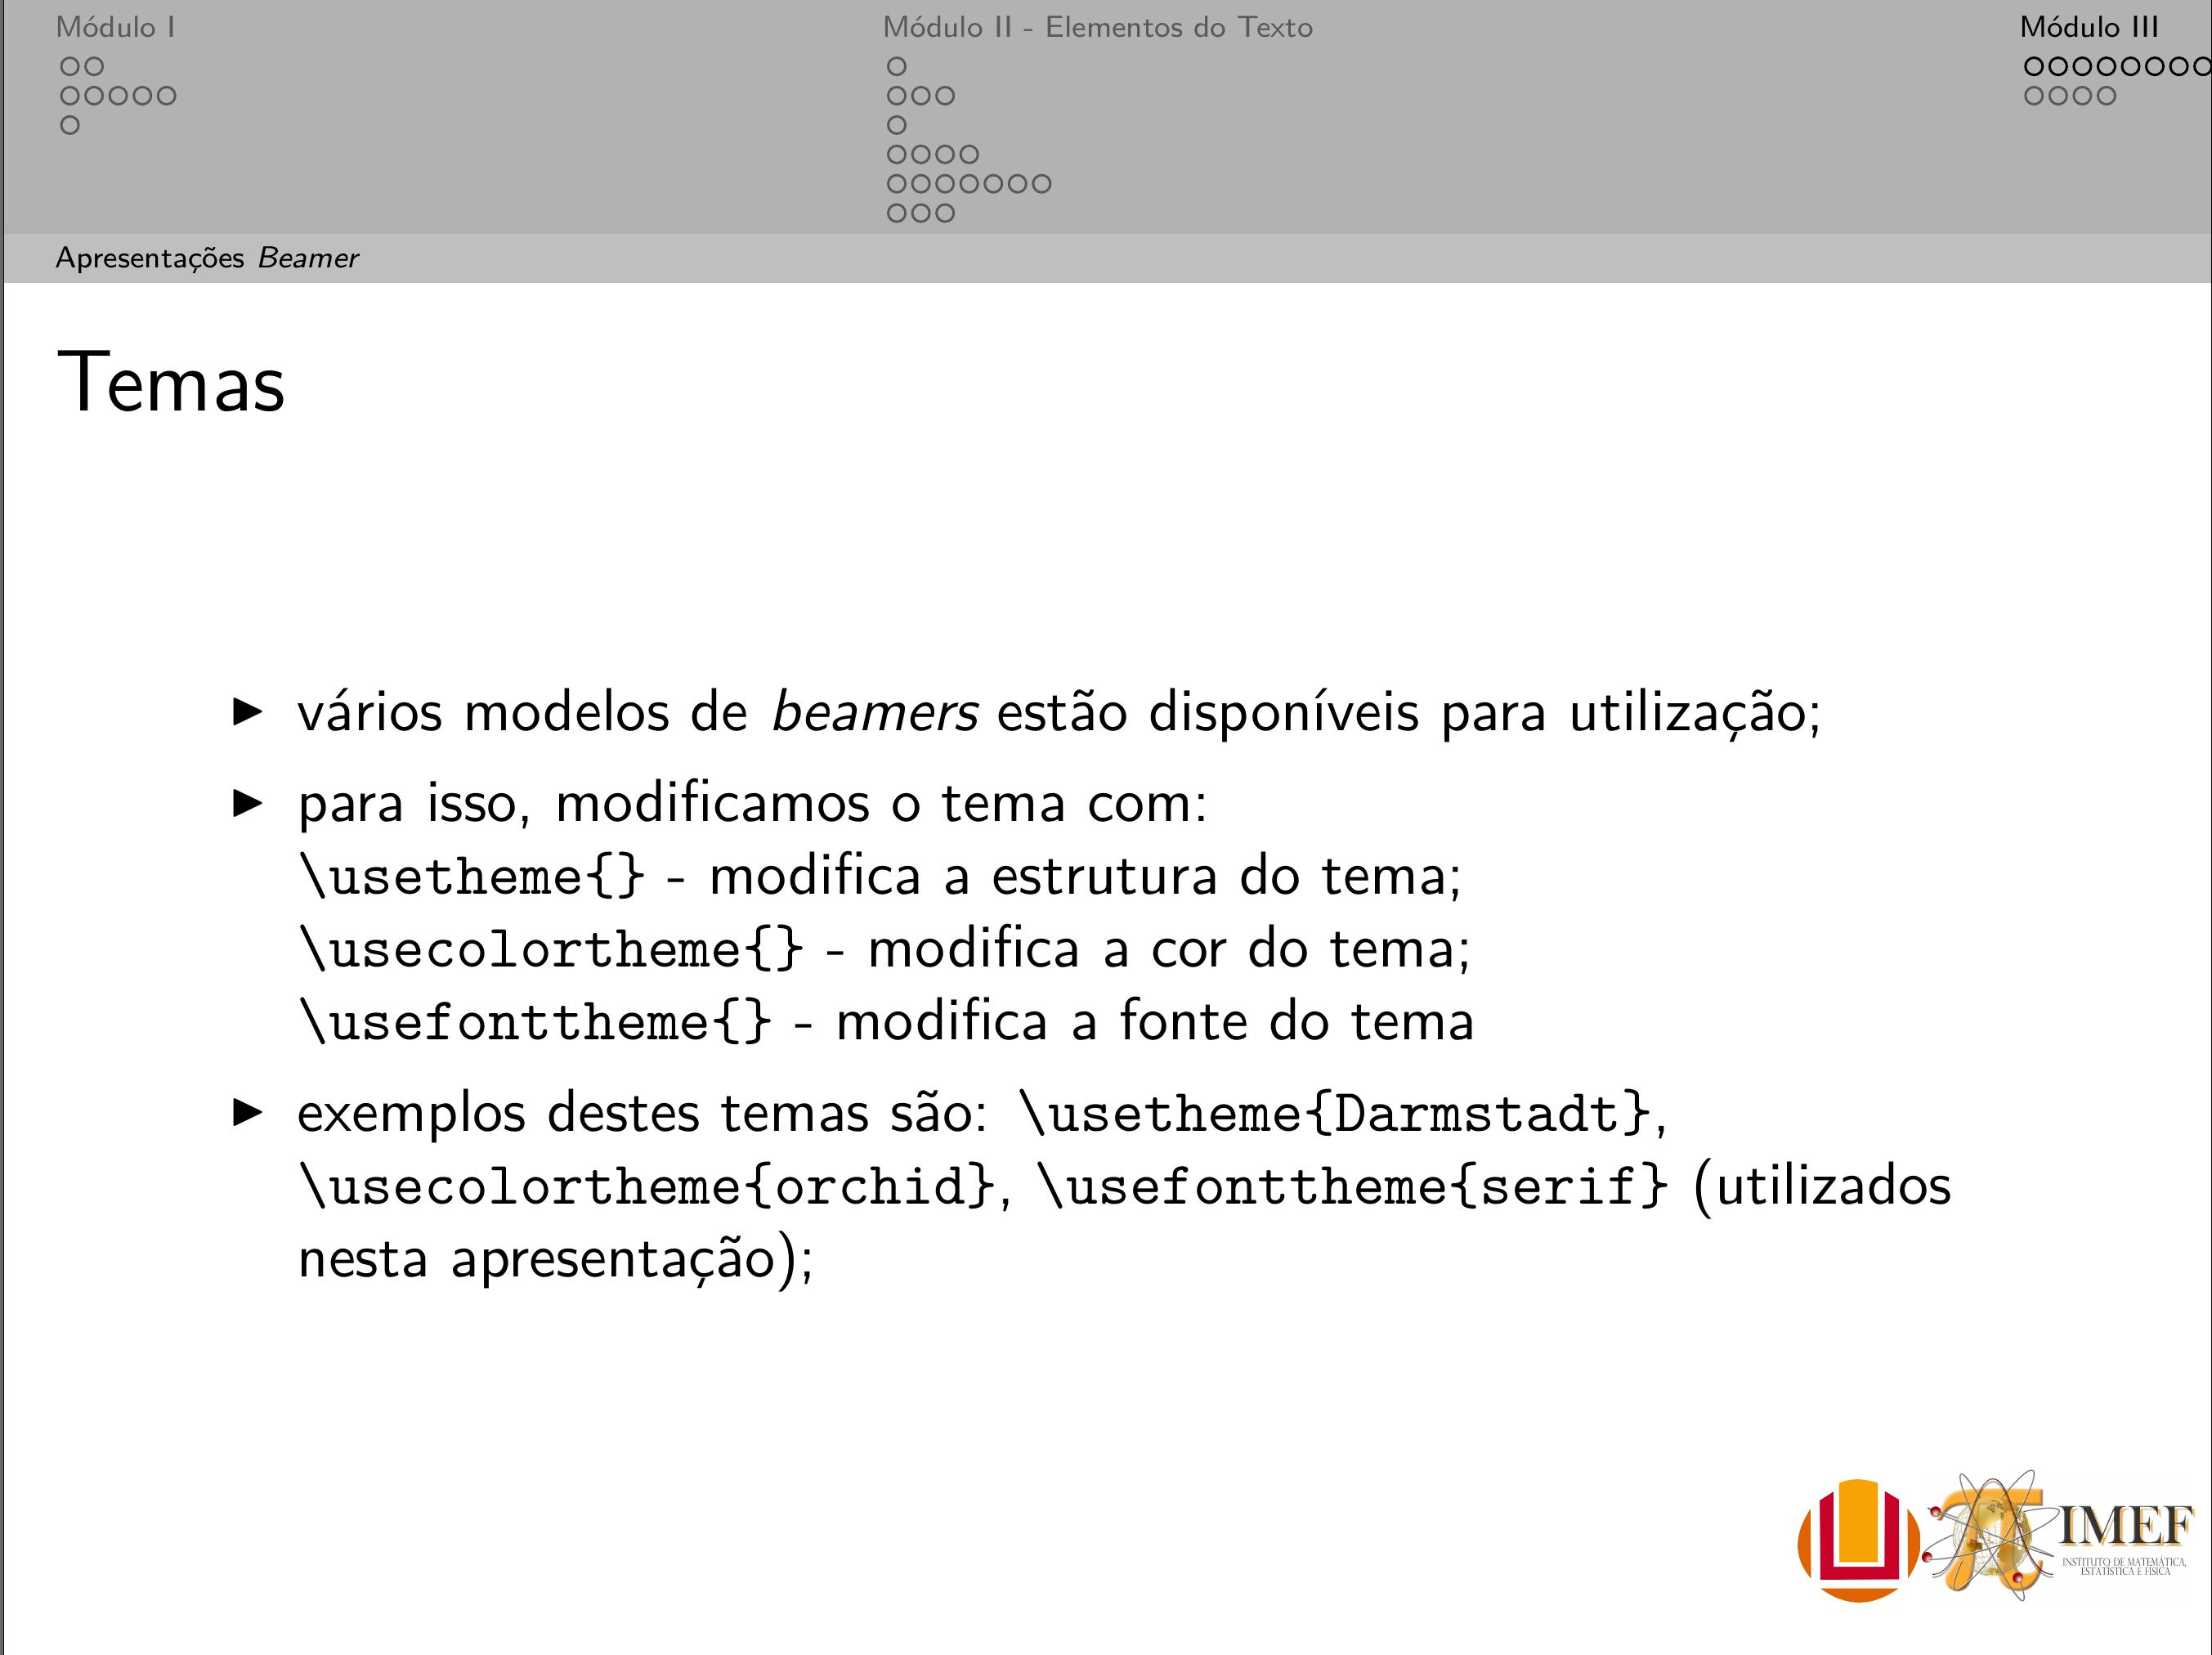
\includegraphics[width=0.40\textwidth]{images/beamer_sze_seau.jpg}
	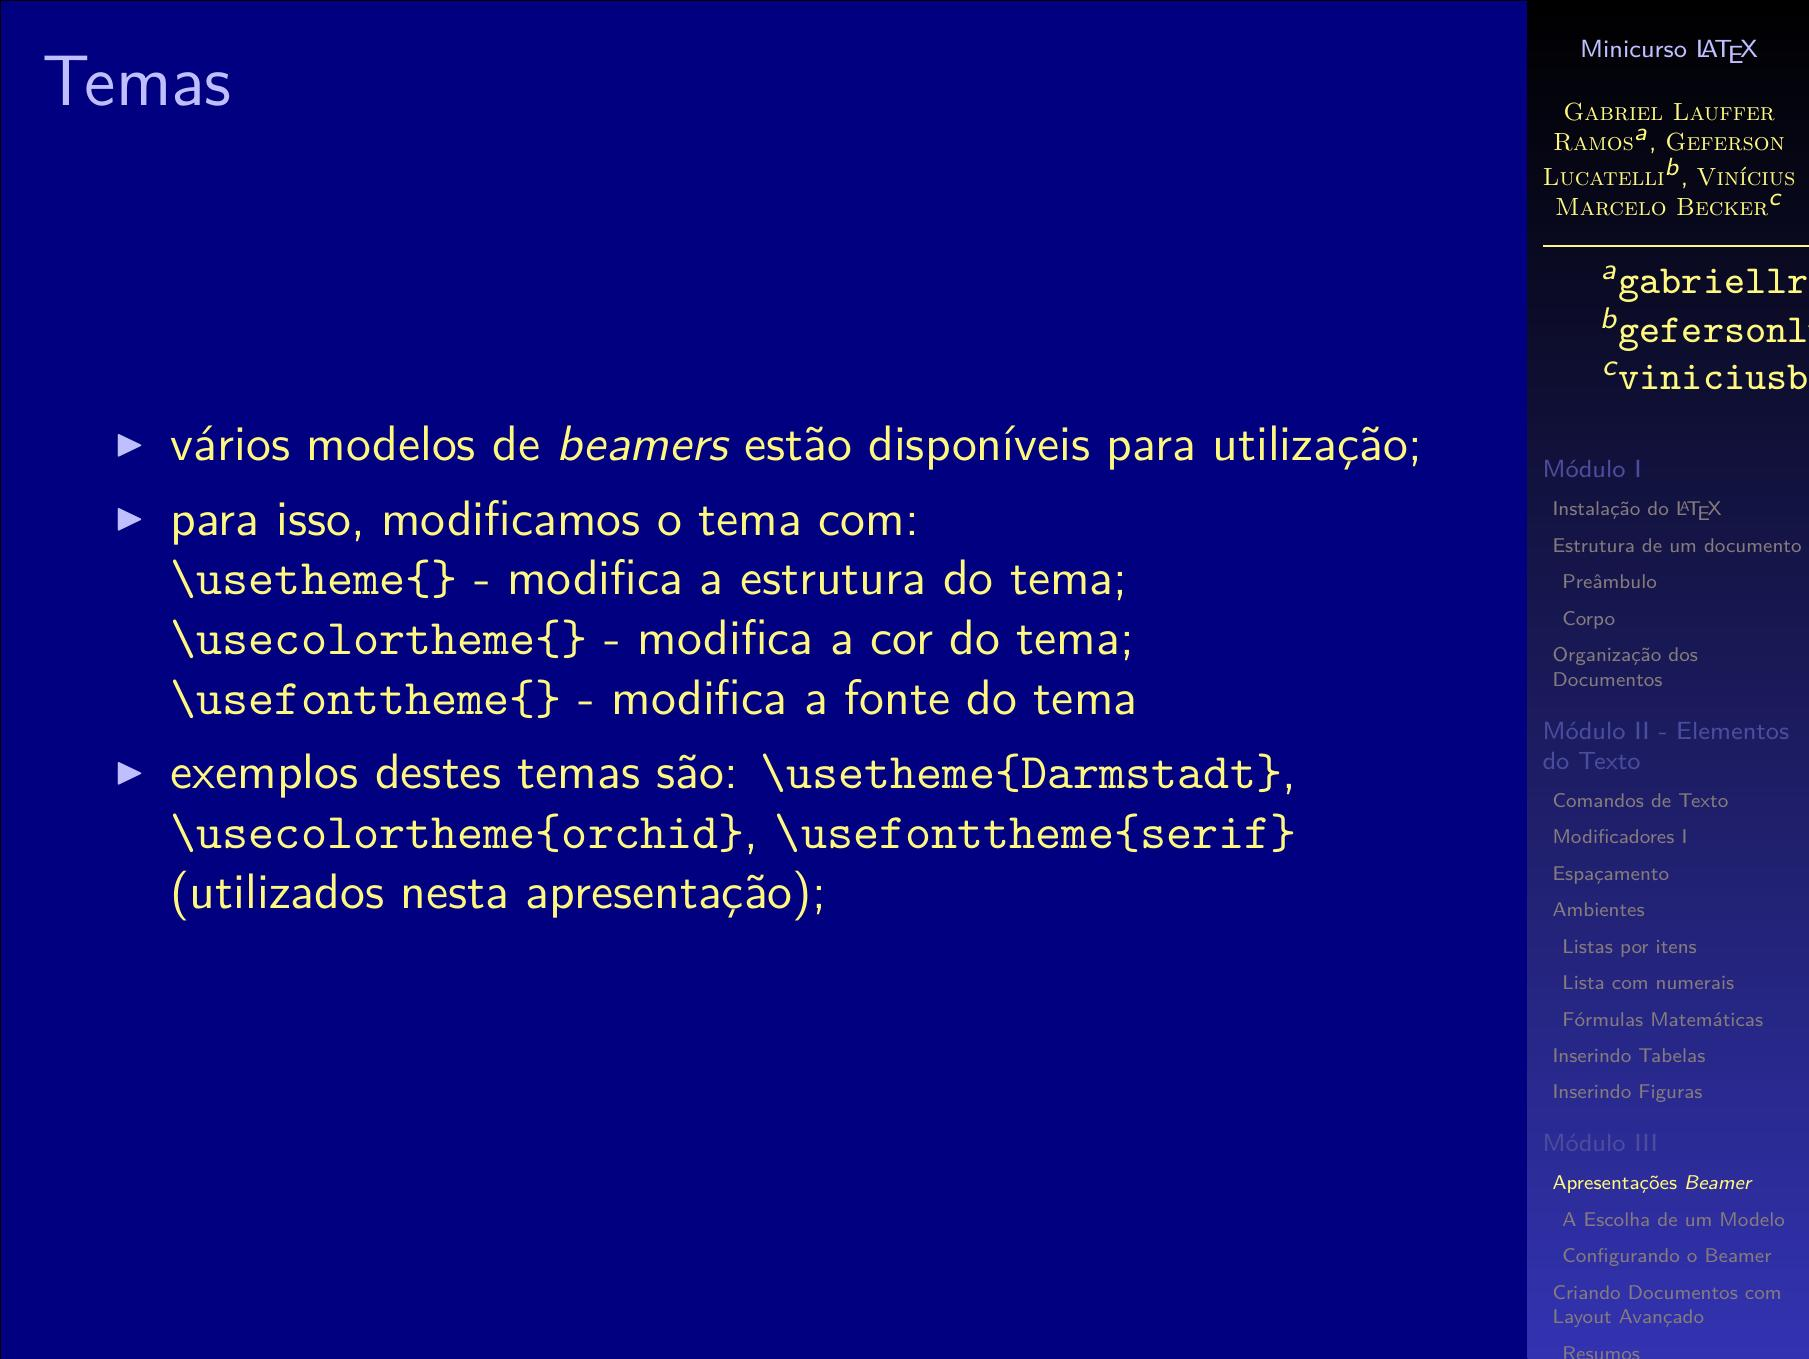
\includegraphics[width=0.40\textwidth]{images/beamer_marb_alb.jpg}\\
	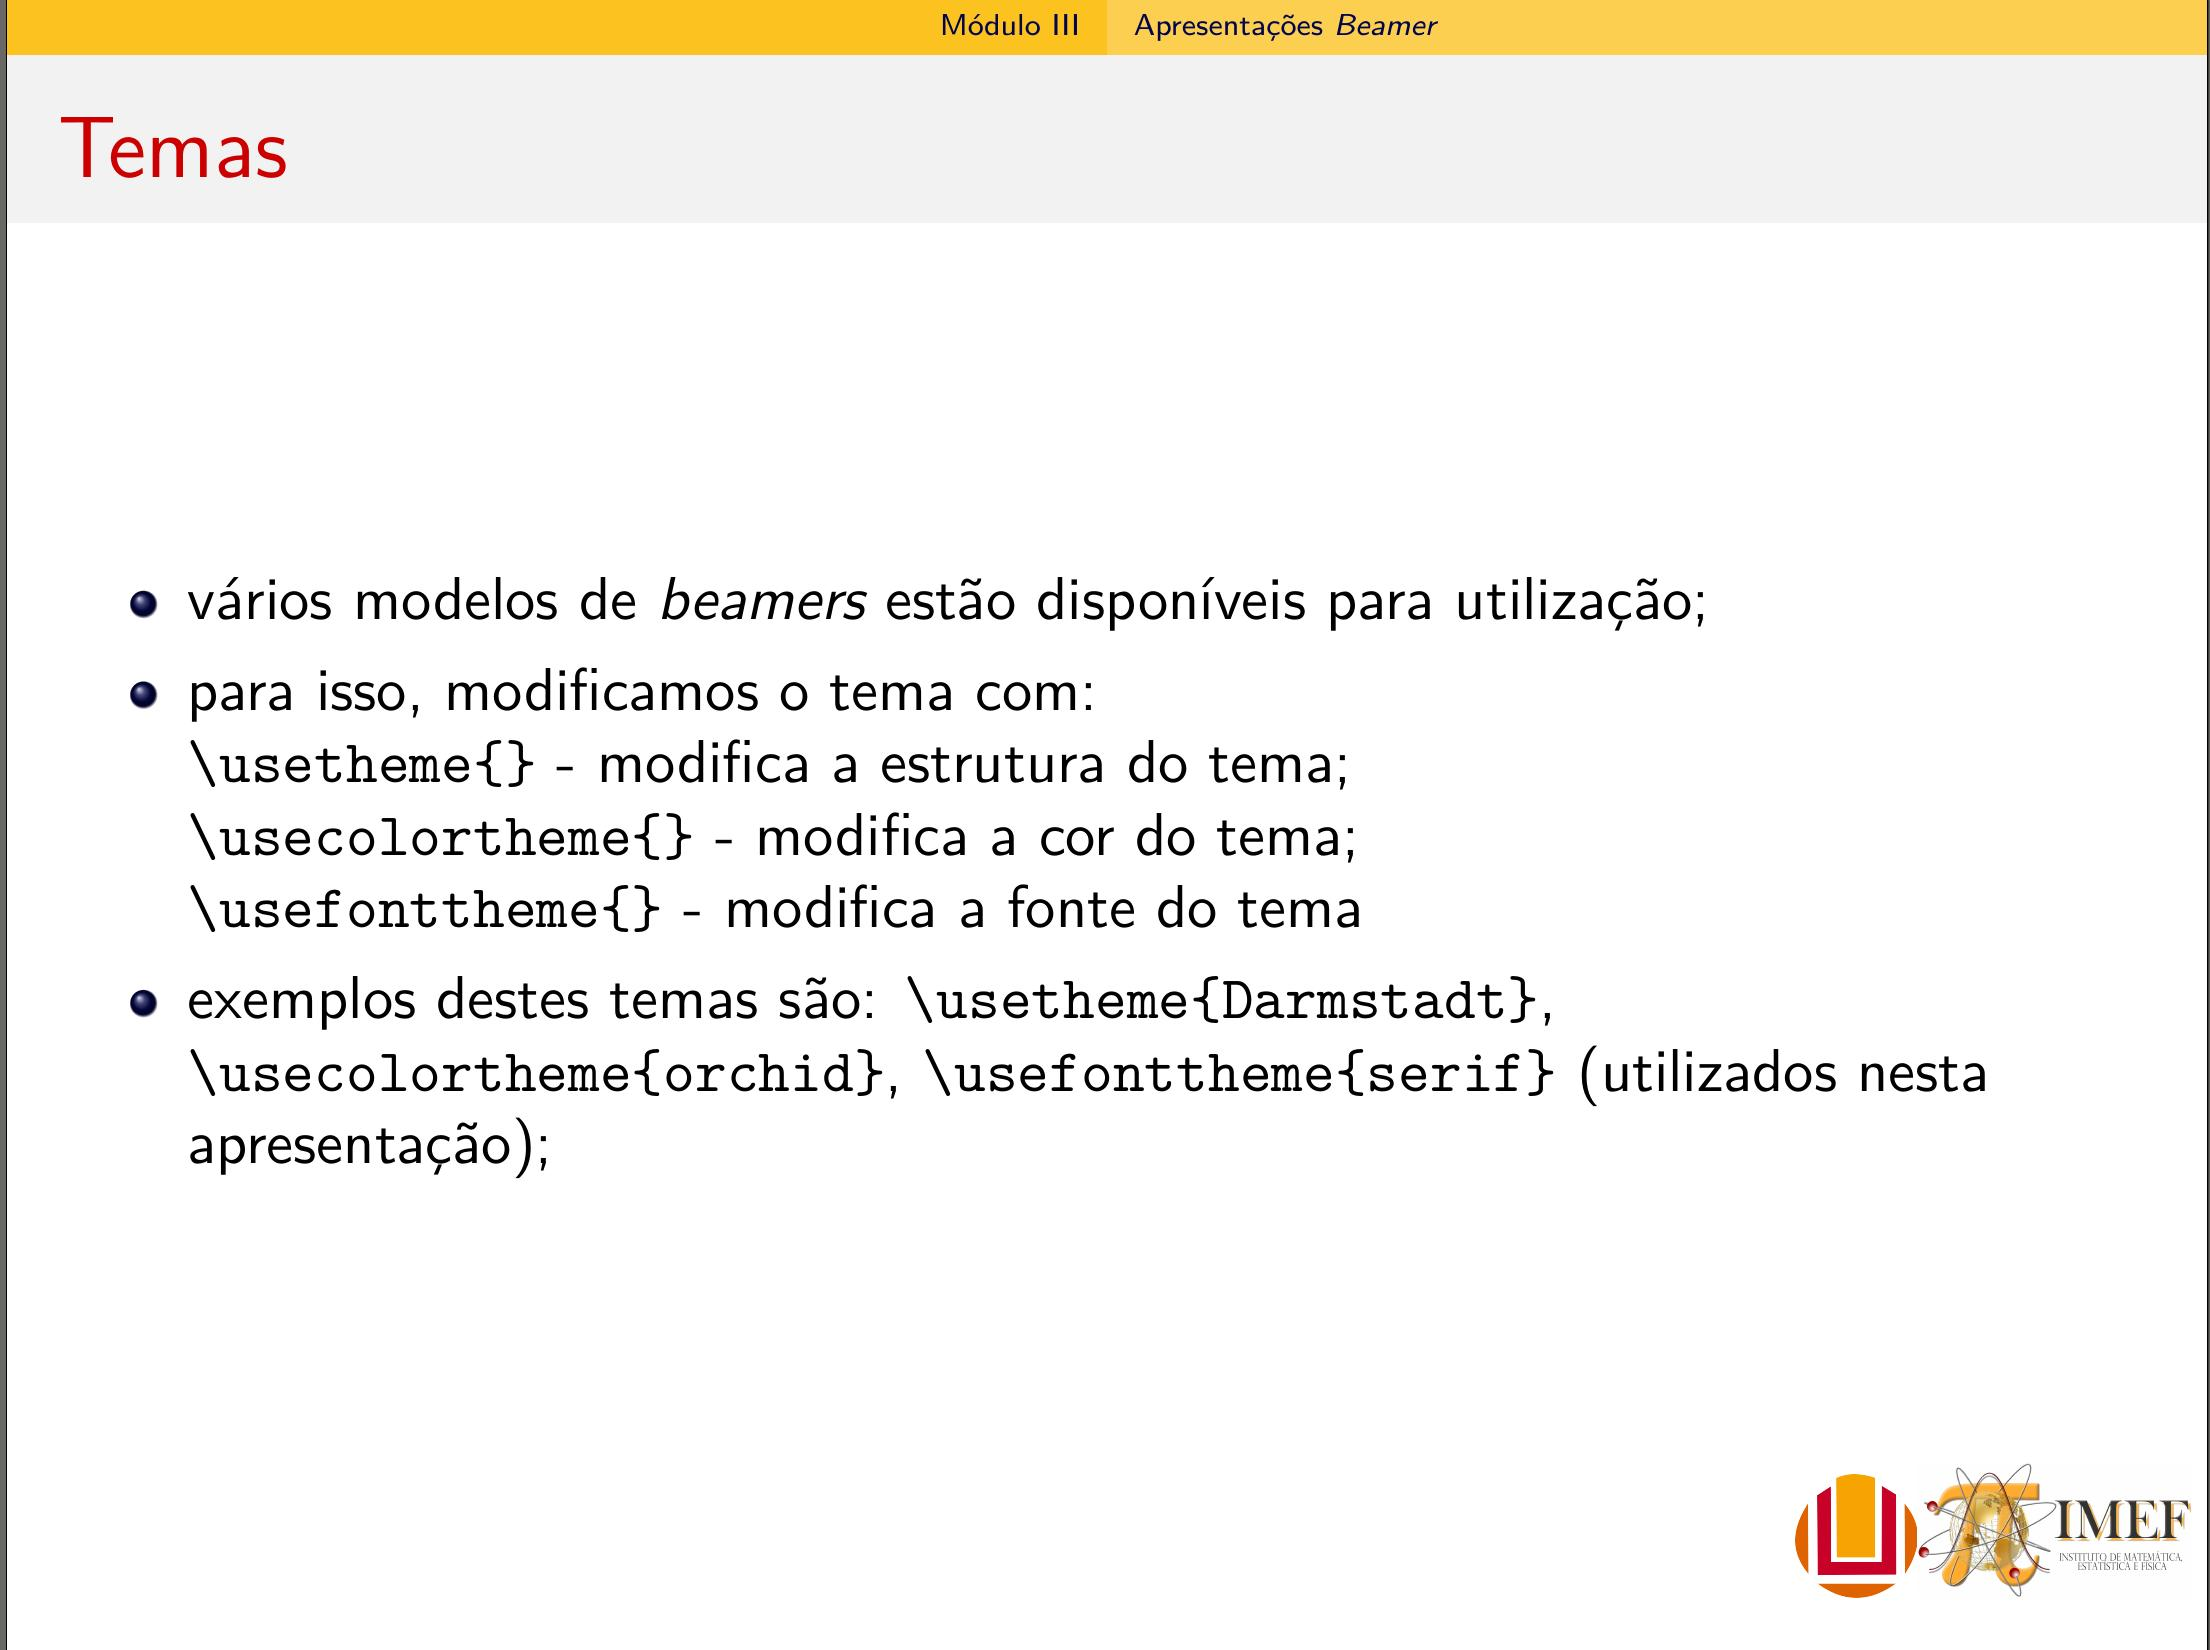
\includegraphics[width=0.40\textwidth]{images/beamer_cambr_crane.jpg}
	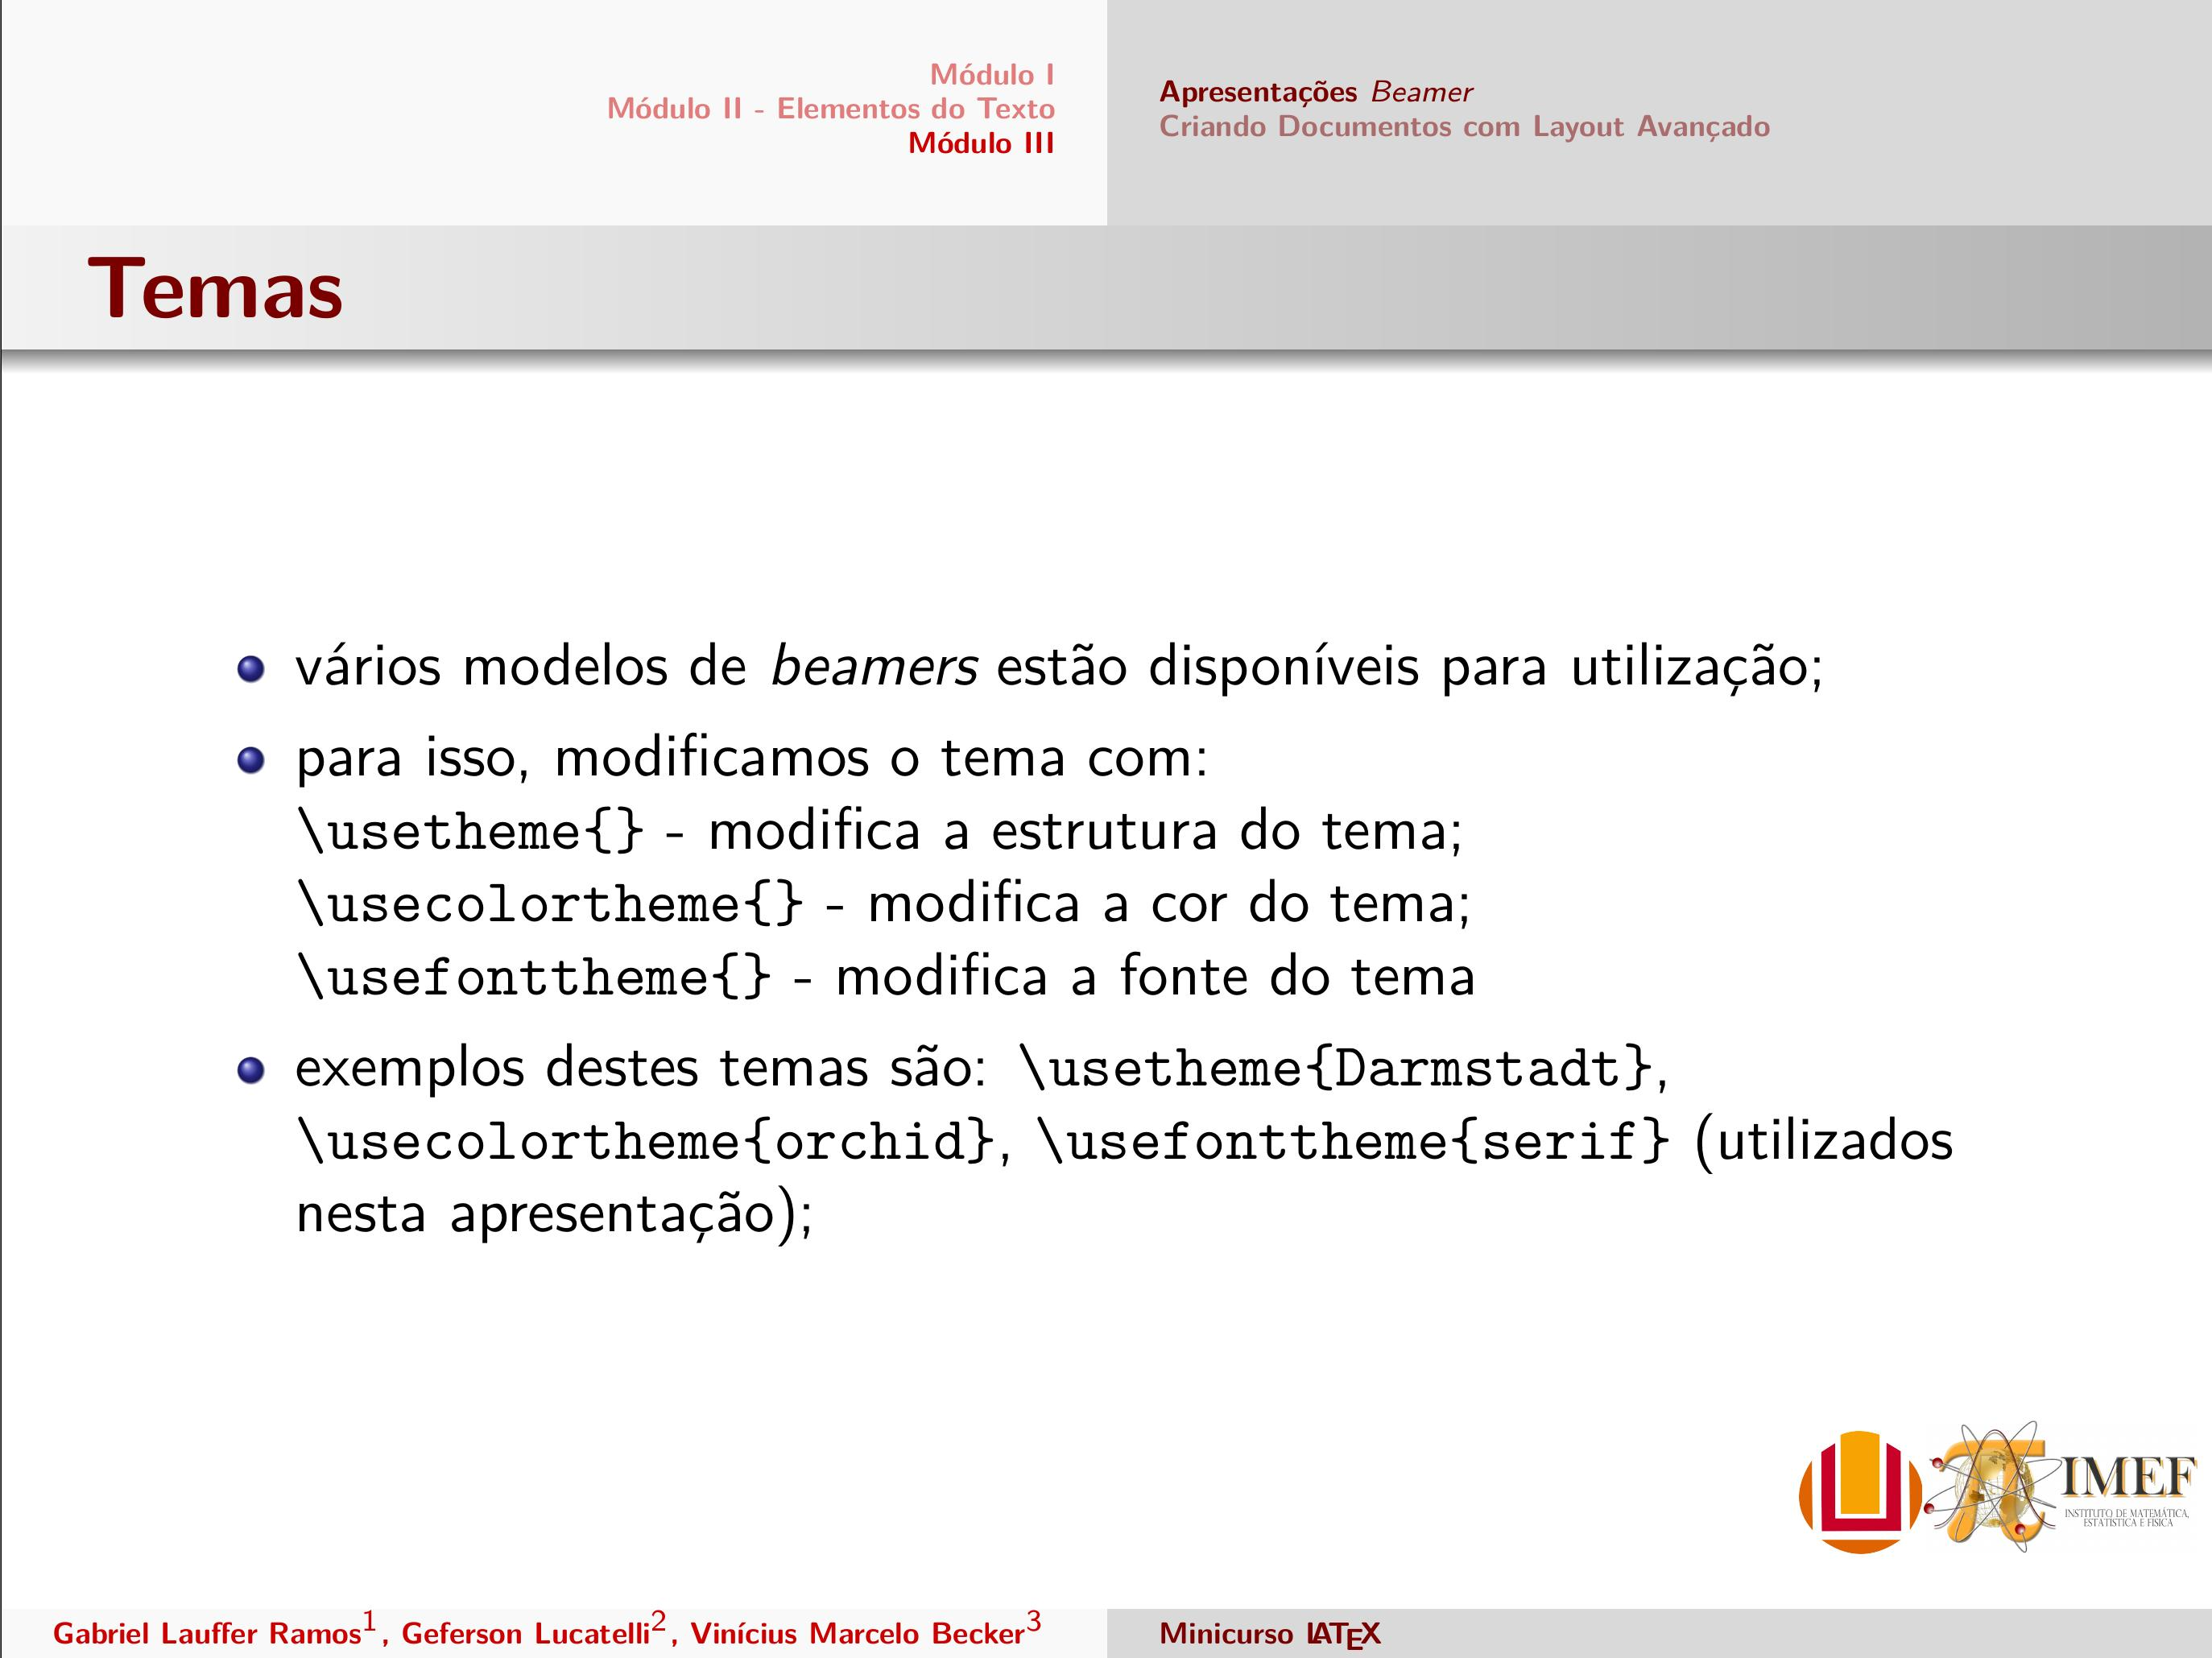
\includegraphics[width=0.40\textwidth]{images/beamer_beav_war.jpg}
\end{figure}
\end{frame}




{\fontsize{5pt}{4.0}\selectfont
\begin{frame}[fragile]{{\sc Temas - este} \texttt{beamer}}
\begin{verbatim}
\documentclass[c]{beamer}
\mode<presentation>
{
\usetheme[progressbar=frametitle]{metropolis}
\usecolortheme{default
\usefonttheme{serif}
\setbeamertemplate{navigation symbols}{}
\setbeamertemplate{caption}[numbered]
\setbeamercovered{transparent}
} 

\usepackage[utf8]{inputenc}
\usepackage[brazil]{babel}
\usefonttheme{serif}
\usepackage{ebgaramond-maths}
\usepackage{amsmath,amssymb}
\usepackage{graphicx}
\usepackage{float}
\usepackage{caption}
\usepackage{subcaption}
\captionsetup[figure]{labelfont=sc}
\usepackage{multicol}
\usepackage{verbatim}

\title{{\sc Introdução ao \LaTeX}}
\subtitle{Módulo 3: Apresentações de slides, Referências e outras técnicas.}
\date{\today}
\author{	{\large XI Semana Acadêmica da Física}\\
Geferson {\sc Lucatelli}\inst{1}\footnote{\texttt{gefersonlucatelli@gmail.com}},
Fernanda Vanucci {\sc Sica}\inst{1}\footnote{\texttt{fervanucci@gmail.com.com\\[0.5cm]}}}
\institute{{\Large Universidade Federal do Rio Grande} \\[0.3cm]
{\inst{1}\large Instituto de Matemática, Estatística e Física
}}
\titlegraphic{\hfill

\includegraphics[height=1.5cm]{images/furg.png}\\[2.5cm]{
\hspace*{8cm}
\includegraphics[height=1.5cm]{images/imef2.png}}
\hspace*{8.5cm}
\includegraphics[height=2.0cm]{images/safis_logo.jpg}
}

\setbeamertemplate{section in toc}{\hspace*{1em}\inserttocsectionnumber.~\inserttocsection\par}
\setbeamertemplate{subsection in toc}{\hspace*{2em}\inserttocsectionnumber.\inserttocsubsectionnumber.~\inserttocsubsection\par}

\begin{document}
\maketitle
\end{verbatim}
\end{frame}
}

\section{Referências}
\plain{Lidando com referências}

\plain{Fazer juntos no Texstudio!}

%\begin{frame}[fragile]{\sc Referências}
%	\begin{itemize}
%		\setlength\itemsep{0.3cm}
%		\item 
%	\end{itemize}
%\end{frame}


\plain{Fim do Módulo II!!!\\
Dúvidas?}



%\section{Referências}



\begin{frame}[allowframebreaks]{References}
\bibliography{references}
\nocite{*}
\end{frame}
\plain{Gracie!}

} 

\end{document}


